%%%  Ukázkový text a dokumentace stylu pro text závěrečné (bakalářské a
%%%  diplomové) práce na KI PřF UP v Olomouci
%%%  Copyright (C) 2012 Martin Rotter, <rotter.martinos@gmail.com>
%%%  Copyright (C) 2014 Jan Outrata, <jan.outrata@upol.cz>


%%  Pro získání PDF souboru dokumentu je třeba tento zdrojový text v
%%  LaTeXu přeložit (dvakrát) programem pdfLaTeX.

%%  V případě použití programu BibLaTeX pro tvorbu seznamu literatury
%%  je poté ještě třeba spustit program Biber s parametrem jméno
%%  souboru zdrojového textu bez přípony a následně opět (dvakrát)
%%  přeložit zdrojový text programem pdfLaTeX.

%%  Postup získání Postscriptového souboru je popsán v dokumentaci.


%%  Třída dokumentu implementující styl pro závěrečnou práci. Vybrané
%%  nepovinné parametry (ostatní v dokumentaci):

%%  'master' pro sazbu diplomové práce, jinak se sází bakalářská práce

%%  'program=kód' pro Váš studijní program/obor (specializaci), kódy
%%  pro diplomovou práci 'infoi' pro Informatiku (Obecná informatika),
%%  'infui' pro Informatiku (Umělá inteligence), 'ainfpst' pro
%%  Aplikovanou informatiku (Počítačové systémy a technologie), 'uinf'
%%  pro Učitelství informatiky pro střední školy, 'binf' pro
%%  Bioinformatiku, 'inf' pro Informatiku (bez specializací) a 'ainf'
%%  pro Aplikovanou informatiku (bez specializací), jinak je výchozí
%%  ainfvs pro Aplikovanou informatiku (Vývoj software), a pro
%%  bakalářskou práci 'infoi' pro Informatiku (Obecná informatika),
%%  'itp' pro Informační technologie v prezenční formě, 'itk' pro
%%  Informační technologie v kombinované formě, 'infv' pro Informatiku
%%  pro vzdělávání, 'binf' pro Bioinfomatiku, 'inf' pro Informatiku
%%  (bez specializací), 'ainfp' pro Aplikovanou informatiku (bez
%%  specializací) v prezenční formě, 'ainfk' pro Aplikovanou
%%  informatiku (bez specializací) v kombinované formě, jinak je
%%  výchozí infpvs pro Informatiku (Programování a vývoj software)

%%  'printversion' pro sazbu verze pro tisk (nebarevné logo a odkazy,
%%  odkazy s uvedením adresy za odkazem, ne odkazy do rejstříku),
%%  jinak verze pro prohlížeč

%%  'biblatex' pro zapnutí podpory pro sazbu bibliografie pomocí
%%  BibLaTeXu, jinak je výchozí sazba v prostředí thebibliography

%%  'language=jazyk' pro jazyk práce, jazyky english pro anglický,
%%  slovak pro slovenský, jinak je výchozí czech pro český

%%  'font=sans' pro bezpatkový font (Iwona Light), jinak výchozí
%%  patkový (Latin Modern)

\documentclass[
%  master,
  program=inf,
%  printversion,
biblatex=false,
%  language=english,
%  font=sans,
sourcecodes=true,
joinlists=true,
  figures=true,
  tables=true,
  glossaries=true,
  index=false
]{kidiplom}

\graphicspath{{./img/}}

%% Informace pro úvodní strany. V jazyku práce (pokud není v komentáři
%% uvedeno česky) a anglicky. Uveďte všechny, u kterých není v
%% komentáři uvedeno, že jsou volitelné. Při neuvedení se použijí
%% výchozí texty. Text pro jiný než nastavený jazyk práce (nepovinným
%% parametrem language makra \documentclass, výchozí český) se zadává
%% použitím makra s uvedením jazyka jako nepovinného parametru.

%% Název práce, česky a anglicky. Měl by se vysázet na jeden řádek.
\title{Bot na platformě Discord}
\title[english]{Bot on Discord platform}

%% Volitelný podnázev práce, česky a anglicky. Měl by se vysázet na
%% jeden řádek. Výchozí je prázdný.


%% Jméno autora práce. Makro nemá nepovinný parametr pro uvedení
%% jazyka.
\author{Lukáš Netřeba}

%% Jméno vedoucího práce (včetně titulů). Makro nemá nepovinný
%% parametr pro uvedení jazyka.
\supervisor{Mgr. Roman Vyjídáček}

%% Volitelný rok odevzdání práce. Výchozí je aktuální (kalendářní)
%% rok. Makro nemá nepovinný parametr pro uvedení jazyka.
%\yearofsubmit{\the\year}

%% Anotace práce, včetně anglické (obvykle překlad z jazyka
%% práce). Jeden odstavec!
\annotation{Obsahem práce je vytvoření Bota pro uživatele a komunity nacházející se
na komunikační platformě Discord. Tato aplikace umožní bota používat pro správu komunit, 
nastavení jejich pravidel, pravomocí a moderace chatu. Bot umožní vytvářet a 
organizovat události, na které se uživatelé z komunit budou moci přihlásit a být upozorněni 
před jejich začátkem. Bude moct zprostředkovávat audio přehrávač skrze hlasové kanály na serverech.}

\annotation[english]{Content of this thesis aims to create a Bot for users and communities on Discord platform.
Application will provide management for those communities with their own set of rules, permissions and chat moderation.
The bot will take care of creating and organizing scheduled events for community users that can participate in and be notified
just before the event starts. The bot will also mediate an audio player in voice channels on the servers.}

%% Klíčová slova práce, včetně anglických. Oddělená (obvykle) středníkem.
\keywords{Discord, nástroj pro správu, Python, Bot, audio přehrávač, události}
\keywords[english]{Discord, administration tool, Python, Bot, audio player,
scheduled events}

%% Volitelná specifikace příloh textu práce, i anglicky. Výchozí je '1
%% CD/DVD'.
%\supplements{jedno kulaté placaté CD/DVD s malou kulatou dírou uprostřed}
%\supplements[english]{one round flat CD/DVD with a small round hole in the middle}

%% Volitelné poděkování. Stručné! Výchozí je prázdné. Makro nemá
%% nepovinný parametr pro uvedení jazyka.
\thanks{Chtěl bych poděkovat svému vedoucímu práce, panu Mgr. Romanu Vyjídáčkovi, za to,
že mi umožnil zpracovat toto téma a za jeho odbornou pomoc při jeho zpracování.
Dále bych chtěl poděkovat svým blízkým a kolegům, kteří byli se mnou trpěliví a motivovali 
mě k vypracování práce.}

%% Cesta k souboru s bibliografií pro její sazbu pomocí BibLaTeXu
%% (zvolenou nepovinným parametrem biblatex makra
%% \documentclass). Použijte pouze při této sazbě, ne při (výchozí)
%% sazbě v prostředí thebibliography.
% \bibliography{bibliografie.bib}

%% Další dodatečné styly (balíky) potřebné pro sazbu vlastního textu
%% práce.
\usepackage{lipsum}
\usepackage{longtable}
\makeglossaries


\newacronym{voip}{VoIP}{Voice over Internet Protocol}
\newacronym{url}{URL}{Uniform Resource Locator}
\newacronym{tos}{ToS}{Terms of Service}
\newacronym{api}{API}{Application Programming Interface}
\newacronym{http}{HTTP}{Hypertext Transfer Protocol}
\newacronym{cli}{CLI}{Command Line Interface}
\newacronym{ui}{UI}{User Interface}
\newacronym{json}{JSON}{JavaScript Object Notation}

\begin{document}

%% Sazba úvodních stran -- titulní, s bibliografickými údaji, s
%% anotací a klíčovými slovy, s poděkováním a prohlášením, s obsahem a
%% se seznamy obrázků, tabulek, vět a zdrojových kódů (pokud jejich
%% sazba není vypnutá).
\maketitle

%% Vlastní text závěrečné práce. Pro povinné závěry, před přílohami,
%% použijte prostředí kiconclusions. Povinná je i příloha s obsahem
%% přiloženého datového média.

%% -------------------------------------------------------------------

\newcommand{\BibLaTeX}{\textsc{Bib}\LaTeX}

%% Úvod
\section{Úvod}
Tato práce se zabývá vytvořením bota pomocí knihovny discord.py v programovacím jazyce Python 
pro komunikační platformu Discord, který
bude sloužit jako nástroj pro komunity ke zlepšení správy nad danou komunitou, jejími pravidly,
nastavením pravomocí pro nově připojené uživatele a jejich následnou kontrolou vůči prohřeškům
z jiných komunit, kde bot mohl problémového uživatele již spatřit a případně tak zavčas
varovat moderátory. Bot umožní vytvoření události s názvem, popiskem a datem konání a evidencí
přihlášených (odmítnutých, nerozhodných) uživatelů na tuto událost a těsně před započetím události je upozorní. Dále
zprostředkuje možnost posílat audio stopu z YouTube přímo do hlasových kanálů na serveru.
V práci jsou rozebrány způsoby, kde lze takovou aplikaci zprovoznit, vlastnosti
každé z možností a realizace jedné z nich.

% V teoretické části jsou popsány požadavky k pochopení a vypracování práce. 
% Tedy způsob, kterým platforma Discord funguje po uživatelské a technické stránce,
% funkcí vlastních aplikací v kontextu s touto platformou a technologiemi
% používanými při jejich vývoji.

% Praktická část se zabývá efektivním návrhem a následnou implementací bota.
Teoretická část textu seznamuje s platformou Discord po její uživatelské a technické stránce, které jsou
nezbytné k pochopení a vypracování práce.
Z uživatelské stránky je zde popsána používaná terminologie v kontextu s touto platformou a také vlastnosti této telekomunikační platformy.
Z technického pohledu je rozebráno, jaké technologie platforma Discord využívá ke své činnosti. Jakým způsobem tyto technologie fungují a jak se dají
využít v rámci vytváření vlastních aplikací.

Praktická část se zabývá efektivním návrhem a následnou implementací bota.
Během návrhu je každá funkcionalita podrobně popsána, jakým způsobem by s ní měl uživatel interagovat, případně popis její cílené činnosti.
Implementace obsahuje vhodnou realizaci navržených funkcionalit bota včetně jejich demonstrace.

Výsledkem práce je funkční aplikace realizující bota, který může být nasazen pro jakoukoliv komunitu na Discordu.
\newpage

%% Teoretická část
\section{Platforma Discord}

%%\newacronym{api}{VoIP}{Voice over Internet Protocol}

Discord je \acrshort{voip} sociální komunikační platforma. Její uživatelé zde mají možnost komunikovat
skrze audiohovor, videohovor, média, soubory a zprávy, a to buď prostřednictvým soukromých chatů
a nebo jako součástí komunit (veřejných, soukromých), kterým se také někdy říká \uv{servery} nebo \uv{guildy}.
Discord je multiplatformní aplikace a běží na operačních systémech Windows, macOS, Linux, Android, iOS či ve webových prohlížečích.
V roce 2021 bylo na Discordu registrováno 350 milionů uživatelů a evidováno 150 milionů aktivních uživatelů denně.

Platforma vznikla jako nápad dvou studentů pro odvětví herního průmyslu, kteří cítili
nedostatky v komunikaci již existujících \acrshort{voip} software se spoluhráči v taktických hrách jako je Final Fantasy XIV.
\cite{ffxiv}
První release Discordu tak byl začátkem roku 2015. Dnes po letech vývoje se používá nejen 
v odvětí herního průmyslu ačkoliv ten stále dominuje. \cite{dc}

Discord je řazen mezi podobné platformy jako jsou např. Microsoft Teams, Microsoft Skype, 
Slack, Teamspeak, Reddit, Facebook Groups, které všechny patří ke komunikačním platformám
s různými rozdíly ve funkcionalitě podle uživatelů na které jsou cíleny.

\subsection{Definice a terminologie}
Discord používá svoji vlastní terminologii, kterou respektuje i tento text a je
používán ve zbytku této práce. Následující seznam vysvětlí nejpodstatnější termíny:

\begin{description}
\item[\texttt{Server}] \hfill \\
Server neboli komunitní server, někdy také označován anglicky slovem {\it guild} v kontextu kódu,
je v uživatelském rozhraní platformy uskupení sdružující uživatele, hlasové
a textové kanály.
  
\item[\texttt{Kanál}] \hfill \\
    Kanál je místo, skrze které mohou uživatelé serveru komunikovat podle jeho typu.
    Existují pouze dva typy kanálů a to {\it hlasové} nebo {\it textové}.
    Textové přenášejí zprávy, média a soubory, zatímco hlasové přenášejí navíc audio
    a video.
  
\item[\texttt{Kategorie}] \hfill \\
    Kategorie je pojmenované uskupení kanálů, které jsou v uživatelském rozhraní platformy
    zobrazeny jako složky. Kategorie mohou obsahovat další kategorie a kanály.
  
\newpage
\item[\texttt{Role}] \hfill \\
    Role je pojmenovaná skupina uživatelů, které mohou být v uživatelském rozhraní platformy
    zobrazeny jako složky. Každá role s sebou nese svoji množinu
    oprávnění a barvu k zobrazení. Role jsou postaveny
    v lineární hierarchii, role tak bývá nadřazena/podřazena jiné roli.
  
\item[\texttt{Emoji}] \hfill \\
    Discord emoji je spojením {\it Unicode} emoji a rozšířením o
    personalizované obrázky definované v rámci
    konkrétního discord serveru.
  
\item[\texttt{Reakce}] \hfill \\
    Reakce je discord emoji, které pomocí interakcí s tlačítkem u libovolné 
    zprávy mohl uživatel nebo bot přidat.

\item[\texttt{Uživatel}] \hfill \\
    Uživatel je osoba, která má vytvořený účet na platformě a může se tak připojit
    k libovolnému serveru. Uživatelé se dělí na dva druhy: {\it člověk} nebo {\it bot}. 
    Když je řečeno slovo uživatel, je tím myšlen druh účtu, který není automatizovaný 
    a stojí za ním skutečný člověk.

\item[\texttt{Bot}] \hfill \\
    Bot je speciální druh uživatele, jehož účet je řízený programem, který komunikuje
    s {\it Discord API} [\ref{discordapi}]. Má přístup k více funkcím než obyčejný uživatel, které může používat
    k různým úkonům. Navíc bývá méně limitován než běžný uživatel v počtu
    zasílaných požadavků do API.

\item[\texttt{Příkaz}] \hfill \\
    Příkaz je textová zpráva napsaná v uživatelském rozhraní v poli pro odesílání
    zpráv. Příkazy se dělí na dva typy, {\it prefixové} nebo {\it lomítkové}. Prefixové
    mají serverem určený speciální symbol, který rozlišuje normální zprávu od příkazové
    k vyhodnocení botem. Tato zpráva je odeslána do chatu jako běžná zpráva. Lomítkový příkaz 
    se neodesílá do chatu jako prefixový příkaz, ale je odchycen v {\it Discord API} a předaný
    botu k obsloužení.

\end{description}


\subsection{Servery a komunity}
Server na platformě Discord je místo, kde se mohou shlukovat uživatelé na jednom místě a komunikovat přes kanály ať hovorem či skrze text.
Server je v uživatelském rozhraní jako kulatá ikonka v jeho levé části klientské aplikace či ve webovém prohlížeči.
Není zde myšleno, že server je výkonný počítač, který obsluhuje požadavky. Discord server, synonymem komunita či guilda, je poskytován a hostován přímo službou discordu jako takovou,
která však běží na fyzických strojích společnosti, které obsluhují několik těchto instancí komunit zároveň.

Na server se může uživatel dostat pouze pomocí pozvánky (vloženou v \acrshort{ui}), která může být krátkým textovým řetězcem připomínajícím hash 
sloužící jako identifikátor pozvánky. Popřípadě \acrshort{url} adresa, kde je zmíněný identifikátor obsažen v jejím parametru. Pozvánka může být
implicitně parametrizována navíc o dobu expirace popřípadě limitem počtu užití. 
Neomezené pozvánky se zpravidla používají pro veřejné servery.

Při vytváření vlastního discord serveru lze v průvodci nastavením najít i šablony pro různé účely, 
které pomohou vytvořit a základně nastavit discord server podle specifických potřeb komunity.

Na serveru se vyskytují kategorie, textové a hlasové kanály a samotní uživatelé serveru a případné
integrace aplikací, které mají programem řízený účet odlišený za jménem pomocí štítku s nápisem \uv{BOT}.

\subsection{Kanály hlasové a textové}
Kanál je prostředník komunikace na platformě, dělí se zpravidla na hlasové a textové, kde soukromý chat je speciální druh kanálu
pouze mezi dvěma uživately. Kanály obecně mají společnou vlastnost, která  
podléhá oprávnění podle rolí nebo také \uv{per user} a nastavením funkčnosti.

Textové kanály mohou být dle oprávnění pro uživatele neviditelné, zamčené pro psaní, zakázané v jiných
směrech např. posílání odkazů, přidávání reakcí, možnost smazat vlastní nebo cizí zprávu, nebo nastavené
na určitý časový limit pro odesílání zpráv.

Hlasové kanály opět podle oprávnění mohou být neviditelné, zaheslované nebo
nastavené na maximální limit současně připojených uživatelů popřípadě
nastavené v kvalitě přenosu audia a videa.

Speciálním případem je komunikace uživatel s jiným uživatelem mimo server přes soukromý chat nebo hovor.
Zde neplatí žádné oprávnění a uživatelé nejsou limitováni oprávněními, které lze aplikovat na role.
Jedinou výjimkou jsou limity nastavené samotnou platformou, mezi které patří znemožnění smazání zpráv druhého uživatele, volitelné znemožnění komunikace
s druhým uživatelem mimo seznam jeho přátel a sdílený společného serveru. Posledním limitem je zde zamezení komunikace, 
kdy příjemce zablokoval odesílatele.

\subsection{Uživatelé, role a pravomoce}
Uživatel je kdokoliv kdo provedl registraci na platformě Discord a zavazuje se
k dodržení podmínek služby, v rámci serveru může mít uživatel jednu či více rolí, které určují
jeho pravomoce.

Role je skupina oprávnění vztahující se pouze na serveru na němž byla vytvořena a může
být přiřazena pouze uživatelům tohoto serveru.

K základní roli, kterou má každý server je role {\it everyone} s výchozím nastavením
oprávnění, které se zpravidla ponechává a vytvářejí se role nové. Pro zpřísnění oprávnění
než je role {\it everyone} bývá zvykem vytvořit novou roli, kterou některý z botů
na serveru nastaví nově příchozím. Tato základní role však slouží v chatové zprávě
pro hromadné označení všech členů serveru pomocí {\it @everyone}.

Existuje jedna role implicitní, kterou je {\it server owner}, dá rozpoznat v 
seznamu uživatelů serveru má uživatel za svým jménem ikonku královské koruny. Role není zobrazena
v seznamu rolí serveru a není možné s ní nijak zacházet, má nejvyšší administrátorské
oprávnění nade všemi.

Role na discord serverech jsou vytvářeny jako pořadový seznam v nastavení serveru,
toto pořadí určuje jejich lineární hierarchii. Což znamená, že role nadřazená může
dělat úkony na roli podřazené.

Pravomoce jsou elementární úkony, které mohou být nastaveny konkrétní roli. Mezi takové
úkony např. patří: právo smazat zprávu, vytvořit pozvánku, vyhodit uživatele, upravit název kanálu, 
upravit nastavení serveru, vytvořit nové role.
Všechny úkony lze vidět v uživatelském rozhraní serveru pro správu rolí.

\subsection{Limitace a předplatné}
Myšleny jsou zde limity, které jsou kladeny na uživatele a komunitní servery
na platformě s možností jejich výběru na základě předplatného. Limitem aplikací pak
rozumíme omezení, které jsou kladeny na účet bota a jeho přístup k informacím platformy.

Některé limity je schopen si uživatel nebo komunitní server navýšit
díky předplatitelům. Pro uživatele se druh předplatného nazývá {\it Nitro Basic} a vylepšená
varianta {\it Nitro}. Předplacený server se nazývá dle její úrovně, které jsou 
{\it Tier 1}, {\it Tier 2} a {\it Tier 3}.

Základní limity, podle tabulky \ref{unpaid}, jsou platné pro 
všechny uživatele a komunitní servery. Většina, až na výjimky (*), nelze ovlivnit zakoupením
předplatného pro server nebo uživatelský účet.
% \clearpage

\begin{table}[h]
  \begin{center}
    \begin{tabular}{|c|c|}
      \hline
      Typ & Limit \\
      \hline
      Počet uživatelů na serveru & 250,000 \\
      Počet online uživatelů na serveru & 5,000 \\
      Počet serverů uživatel smí být členem* & 100 \\
      Počet kategorií na serveru & 50 \\
      Počet kanálů na serveru & 500 \\
      Počet rolí na serveru & 250 \\
      Počet neanimovaných emoji na serveru & 50 \\
      Počet animovaných emoji na serveru & 50 \\
      \hline
    \end{tabular}
  \end{center}
  \caption{\label{unpaid}Základní limity}
\end{table}

Limity s předplatným se v případě předplatného pro uživatele řadí do dvou úrovní,
pro komunitu se předplatné řadí do úrovní tří. Tabulka \ref{paid_user} ukazuje
úrovně předplatného pro uživatele, tabulka \ref{paid_server} ukazuje předplatné úrovně
pro servery.

\begin{table}[h]
  \begin{center}
    \begin{tabular}{|c|c|c|}
      \hline
      Typ & Úroveň 1 & Úroveň 2 \\
      \hline
      Vlastní emoji kdekoliv & Ano & Ano \\
      Vlastní samolepky kdekoliv & Ano & Ano \\
      Velikost souborů & 50MB & 500MB \\
      Vysoké rozlišení videa & Ne & Ano, až 4k@60 \\
      Personalizovaný profil účtu & Ne & Ano \\
      Personalizovaný profil \uv{per server} & Ne & Ano \\
      Odznak předplatitele & Ano & Ano \\
      Vlastní pozadí ve videohovorů & Ano & Ano \\
      Počet serverů uživatel smí být členem & 100 & 200 \\
      Delší zprávy & do 2000 znaků & do 4000 znaků \\
      \hline
    \end{tabular}
  \end{center}
  \caption{\label{paid_user}Úrovně limitů pro předplatitelské účty}
\end{table}

\begin{table}[h]
  \centering
    \begin{tabular}{|c|c|c|c|}
      \hline
      Typ & Úroveň 1 & Úroveň 2 & Úroveň 3 \\
      \hline
      Vlastních emoji serveru & až 100 & až 150 & až 250 \\
      Audio kvalita & až 128Kbps & až 256Kbps & až 384Kbps \\
      Vlastní pozadí v pozvánce & Ano & Ano & Ano \\
      Vlastních samolepek serveru & až 15 & až 30 & až 60 \\
      Animovaná ikona serveru & Ano & Ano & Ano \\
      Kvalita 1080p@30 videa všem & Ano & Ano & Ano \\
      Vlastní ikony rolí & Ne & Ano & Ano \\
      Vlastní banner serveru & Ne & Ano & Ano \\
      Kvalita 1080@60 videa všem & Ne & Ano & Ano \\
      Až 50MB velikost souborů všem & Ne & Ano & Ano \\
      Až 100MB velikost souborů všem & Ne & Ne & Ano \\
      Animovaný vlastní banner serveru & Ne & Ne & Ano \\
      Vlastní odkaz pozvánky & Ne & Ne & Ano \\
      \hline
    \end{tabular}
  % \end{center}
  \caption{\label{paid_server}Úrovně limitů pro předplacené servery}
\end{table}

K limitům patří také \uv{rate limit}, což je maximální počet 
požadavků, které uživatelský účet nebo účet bota může platformě zasílat, bot
má tento limit vyšší. Požadavek je např. odeslání zprávy, vytvoření
pozvánky serveru nebo probíhající audio či videohovor. Při rychlém vyčerpání
přiděleného maximálního počtu požadavků pro určitý časový úsek požadavky nemají 
žádný efekt, dokud neuplyne určitý čas, po kterém se předešlé požadavky automaticky
pokusí sami zopakovat. Nadmírným a úmyslným čerpáním tohoto maximální počtu požadavků
je proti \acrshort{tos} a může dojít k pozastavení nebo odstranění účtu jedince nebo 
komunitního serveru.

\section{Discord Bot}
Discord bot je uživatelský účet, který je kompletně automatizovaný programem, tento
program pak komunikuje prostřednictvým Discord API \cite{discordapi} s platformou, na které provádí
automatické úkony nebo úkony vyvolané uživatelem či prostředím za účelem
vylepšení uživatelské zkušenosti. Platforma komunikuje
s botem skrze WebSocket API \cite{webapi} a předává tak v \uv{realtime} informace bez nutnosti
navazovat neustále nová spojení. Bot si tyto odpovědi ukládá do mezipaměti, 
jedná se tak o rychlý přenos informace mezi platformou a botem.
Druhým směrem bot odpovídá platformě skrze její REST API \cite{restapi}, kde
místo odesílání celých objektů odesílá pouze identifikátory objektů, které má ve své mezipaměti.

Bota si může zřídit jakýkoliv registrovaný uživatel discordu, což může učinit na 
oficiálních webových stránkách platformy, kde svoji aplikaci pojmenuje a vytvoří. 
Vytvořením dostane autorizační token, který poté následně použije ve zdrojovém kódu
podle patřičné implementace Discord API knihovny pro zvolený programovací jazyk.

Clyde bot je bot, jenž nepatří žádnému registrovanému uživateli, ale jedná se o systémového bota
platformy, který je zde pro vylepšení a používání této platformy. Můžeme ho spatřit
na obr. \ref{clyde}, když se pokusíme poslat zprávu uživateli, který nás zablokoval.

% \clearpage
\begin{figure}
  \centering 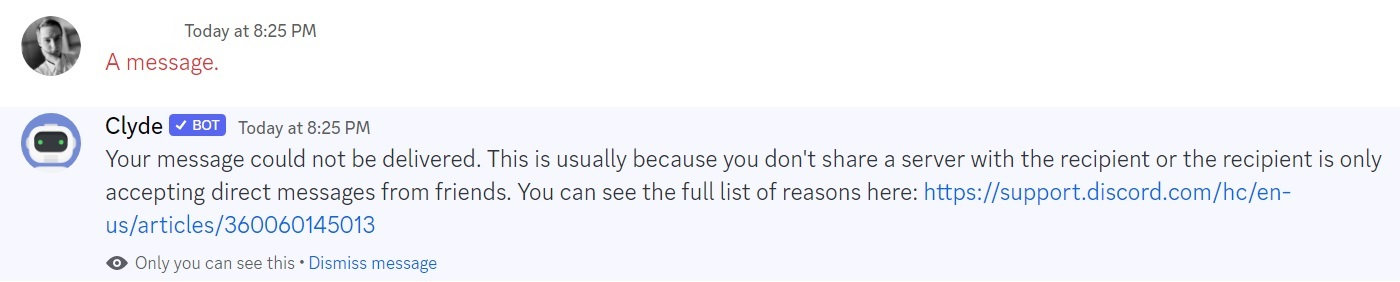
\includegraphics[scale=0.58]{clyde}
  \caption{\label{clyde}Systémový bot platformy Discord}
\end{figure}


\subsection{Ovládání a práce s botem}
Ovládání bota je buď automatické, kdy bot řídí do určité míry svoje ovládání sám, nebo manuální, kdy vyžaduje
vstup od uživatele. Automatické fungují tak, že přes
websocket dostává bot informaci o eventech, které se na platformě stali, třeba uživatel
odeslal zprávu a botu přijde event typu {\it on-message}, pro který ve zdrojovém kódu 
bude vytvořena funkce, která funguje jako {\it callback} a bude spuštěna při tomto
eventu z websocketu. Tyto eventy jsou předdefinované a je na programátorovi, které funkce jako
callbacky vytvoří podle toho, kterým eventům chce jeho aplikace naslouchat. Manuální jsou funkce, které 
definují příkaz prostřednictvým uživatelského rozhraní v chatovacím okně dvěmi způsoby:
prefixovanou zprávou nebo příkaz za lomítkem.

Pokud bot obsahuje funkce, které jsou v příslušném jazyce knihovny Discord API označeny jako event 
a dodržují definované pojmenování, pak budou automaticky skrze knihovnu spuštěny jako callback.

Uživatel bota nemusí v případě úkonů, které reagují na websocketem zaslané eventy, nic dělat. 
Pro úkony, které vyžadují zásah nebo doplnění informací k jejich provedení, musí uživatel tyto úkony
vyvolat manuálně sám přes příkazy prefixové nebo lomítkové.

\subsubsection{Prefixové zprávy}
Prefixové zprávy jsou způsobem komunikace mezi uživatelem a botem, kdy uživatel napíše zprávu do chatu
jako obvykle s rozdílem, že před začátek zprávy dá speciální symbol, který bot
poté rozpozná, která zpráva obsahuje příkaz a která zpráva byla mezi běžnou probíhající 
konverzací na komunitním serveru. Mezi speciální symboly, které se často používají jsou:
{?, !, \&, *}. Tyto symboly jsou vždy na začátku zprávy a následuje za nimi řetězec
znaků, který je definován jako příkaz. Příkaz je pak rozdělen na jeden či více argumentů
pomocí mezer, před první mezerou je tak symbolické jméno příkazu.

\begin{figure}[h]
  \centering 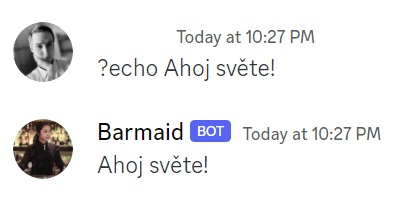
\includegraphics[scale=1]{prefix}
  \caption{\label{prefix_command}Příkaz vyvolaný prefixovanou zprávou}
\end{figure}

Na obr. \ref{prefix_command} můžeme vidět příkaz {\it echo} s jedním argumentem následujícím 
za první mezerou po slově echo. Při implementaci funkce příkazu je vždy možnost pro
poslední argument příkazu posbírat celý řetězec včetně mezer a chápat jej jako jeden argument,
jako tomu je v tomto případě.

Pokud je příkaz s více argumenty, kdy do jednoho argumentu je potřeba dát řetězec 
obsahující i mezery, je potřeba tento řetězec obalit do uvozovek.

\subsubsection{Lomítkové příkazy}
Lomítkový příkaz je novější způsob komunikace uživatele s botem, kdy uživatel předepíše do textového
pole pro odeslání nové zprávy symbol lomítka a zobrazí se mu kontextové menu s výběrem
všech dostupných příkazů.

V uživatelském rozhraní se rozbalí menu s možnostmi příkazů, které jsou definovány v kódu bota. Uživatel vybere příkaz a
je mu našeptáváno jaké hodnoty argumentů je nutné zadat pro úspěšné vykonání
příkazu. Poprvé byly lomítkové příkazy přidány do uživatelského prostředí a do odpovídajích
API koncem roku 2020, v roce 2022 se stali povinností pro boty, kteří musejí
být verifikováni. Verifikovaný bot je zkontrolován vůči práci s citlivými daty uživatelů platformy a jeho
následnému nakládání s nimi. Bot, který
nepřekročí počet 100 komunitních serverů, ke kterým se připojil, nepotřebuje ověření.
O toto ověření lze požádat až při překročení hranice.

\begin{figure}[h]
  \centering 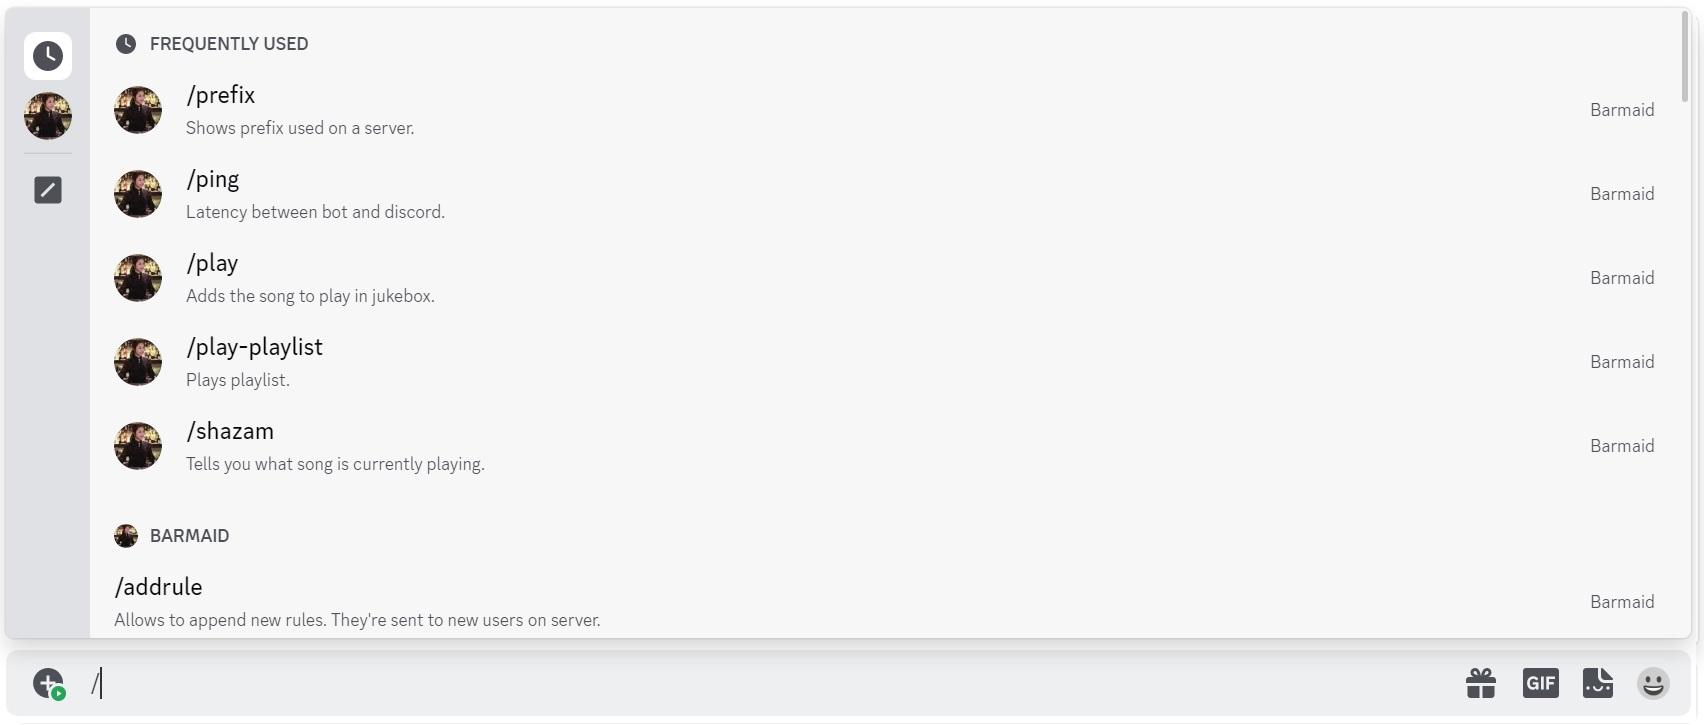
\includegraphics[scale=0.48]{slash}
  \caption{\label{slash_command}Kontextové menu lomítkových příkazů}
\end{figure}

Na obr. \ref{slash_command} vlevo vidíme sloupec, ve kterém nalezneme všechny
boty na daném komunitním serveru. Uprostřed nabídku se všemi příkazy, kde shora jako první
se zobrazují nejčastěji používané příkazy a na konči řádku příkazu vidíme název
bota, kterému příkaz patří. Více botů může mít stejně pojmenovaný příkaz a uživatel
je schopen je rozlišit podle profilové fotky nebo jména bota.

\subsection{Technologie pro vývoj}
Pro komunikaci s Discord platformou má sama platforma své vlastní \acrshort{api}, k počátku roku
2023 se datuje už {\it 10.} verze. Dá se používat ještě verze předešlá, verze {\it 6-8} jsou 
nyní zastaralé a verze {\it 1-5} jsou již zrušené. \cite{discordapi} Komunikovat s tímto API
napřímo je náchylné na chyby programátora při implementaci, které mohou způsobit
nechtěné přetěžování API, které může vyústit k zablokování této komunikace platformou
nebo dokonce účtu bota či samotného uživatele vlastnícího tohoto bota. Od těchto strastí
s verzí a správnou komunikací nás abstrahují knihovny pro práci s API platformy Discord.
Knihovny jsou napsány jako \uv{wrapper} v patřičném programovacím jazyce usnadnující 
práci s API a ošetřují jeho nebezpečného zacházení. Další knihovny pro vybraný programovací
jazyk mohou pomoci při komunaci bota s webovými stránkami na internetu, databází a 
dalšími službami pro vlastní dovednosti bota.

\subsubsection{Discord API}
Discord API je preferovaný způsob komunikace mezi botem a platformou Discord. Umožňuje snadné, rychlé
a bezpečné vytvoření bota pro komunikaci s platformou přes dva základní prvky:
{\it WebSocket API} a {\it REST API}.
Na obr. \ref{discordapi} převzatého z článku \cite{restapi} je vidět průběh 
komunikace, kdy platforma vlevo komunikuje
ve směru bota pomocí WebSocket API \cite{webapi}, a bot vpravo ve směru platformy pomocí volání REST API. \cite{restapi}

\begin{figure}[h]
  \centering 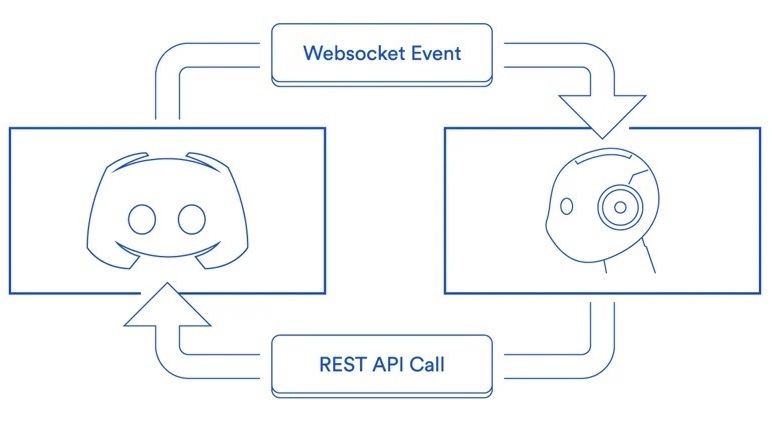
\includegraphics[scale=0.9]{discordapi}
  \caption{\label{discordapi}Způsob komunikace bota a platformy \cite{restapi}}
\end{figure}

\subsubsubsection{WebSocket API}
WebSocket API je používán při přijímání eventů, při změně stavu na platformě, ze serverových strojů platformy Discord. Komunikace
je navázána mezi platformou a botem skrze websocket, který je jednou vytvořen a umožňuje přenášet informace v 
\uv{realtime}, eliminuje se tím potřeba pro každý přenos informace vytvořit nové spojení 
a vzniká tak velmi rychlý způsob přenosu informací.

Mezi eventy, které se přenáší z platformy botu jsou například: uživatel zaslal zprávu, uživatel upravil zprávu, uživatel smazal zprávu, 
uživatel se připojil ke komunitě, uživatel připnul zprávu, uživatel vytvořil vlákno ve zprávě, 
uživatel se připojil k hovoru, uživatel si ztlumil mikrofon v hovoru.

Během přenosu informace o eventu jenž nastal, jsou spolu s ním předávány objekty 
{\it zpráv}, {\it uživatele}, {\it místnosti}, {\it komunitního serveru}
obsahující jejich úplné informace. Po úspěšném přenosu informace o tom, že nastal event, si bot ukládá
všechny informace o objektech do {\it cache}, se kterými je poté schopen pracovat své
pro úkony a odesílá odpovědi s výstupy do {\it REST API}.

\subsubsubsection{REST API}
Akce, které je bot schopen provést, musí učinit přes volání {\it REST API}. Bot je také
schopen si skrze {\it REST API} vyžádat získání informací, ale to není zpravidla kvůli efektivitě přenosu
používáno, neboť většinu potřebných informací v aktuálním stavu, již dostal z websocketu a má je uložené ve své
{\it cache}. 

Bot z této cache vytáhne objekty, se kterými potřebuje pracovat a při
provedení změn nad nimi odesílá do {\it REST API} pouze {\it identifikátor} objektu a změnu, kterou provedl.
Neodesílá tak znovu celý objekt z důvodu rychlosti a případnému zahlcení API.

Identifikátor objektu je celé přirozené číslo, pod kterým si platforma je schopna
najít objekt, kterému patří. V případě bota si i bot je schopen pomocí identifikátoru
dohledat objekt, kterému patří, ale s omezením, že objekt se musí nacházet v jeho cache. Nemůže tak například
získat objekt komunitního serveru jehož bot není členem i kdyby znal jeho identifikátor, protože
takový objekt mu websocket s tímto identikátorem nikdy nezaslal.

\subsubsection{Asyncio}
Asyncio je knihovna pro práci s asynchronním programováním používaném při komunaci klient-server, kdy nějaký čas trvá než
se informace přenese a dostaví se její odpovědi, pro využití procesorového času efektivně namísto čekání se vykonává
něco jiného zatímco se čeká než odpověď dorazí. \cite{asyncio} Asyncio, přesněji asyncIO je zkratka za asynchronous
input/output, technologie která se stará o efektivní hospodaření s procesorovým časem při operacích, jenž
mají delší efekt jako právě komunikace po síti.

Tato technologie dává možnost tzv. \uv{single threaded} procesům zdánlivě vykonávat více operací současně.
%jako jsou například samotné webové prohlížeče s {\it JavaScriptem}.
Dlouho trvající operace nejprve všechny naráz jednu po druhé spustí a 
po vyčkání vrací v žádaném pořadí odpovědi po provedení operace, než aby se sekvenčně spustila jedna operace zvlášť a vyčkalo se na 
její dokončení než se spustí v sekvenci další dlouhotrvající operace.
% zkrátka spustíme více dlouho trvajících věcí postupně a pak čekáme na všechny z nich zároveň.

Program má pouze jedno vlákno označované též jako {\it main thread} a tedy jeden {\it execution stack}, kde 
může vykonávat pouze jednu operaci. Při asynchronním programování požadavek jako je získání dat z 
webové stránky by blokoval execution stack po celou dobu čekání na odpověď. Namísto toho předává tento svůj požadavek
do {\it event loopu} a z execution stacku se tím funkce odstraní a na její místo se ukládá návratová adresa, kam se tato funkce po vykonání event loopem navrátí.
Funkce je tedy {\it callback} funkcí.
Event loop se postaraná o obsloužení tohoto požadavku a spustí jej. Po dokončení požadavku se skrze callback vrací odpovědi
požadavku zpátky do execution stacku main threadu.

\begin{figure}[h]
  \centering 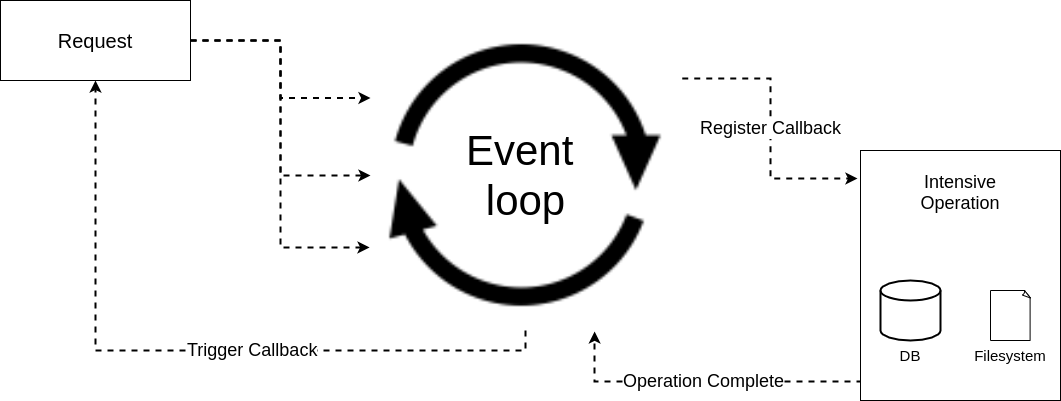
\includegraphics[scale=0.38]{loop}
  \caption{\label{asyncio}Asynchronní programování s jedním procesem \cite{loop}}
\end{figure}

Na obr. \ref{asyncio} vlevo vidíme request z main threadu programu předaný event loop
smyčce starající se o časově náročné input/output operace znázorněné vpravo, po jejich dokončení
se vrací výsledek operace zpět přes callback do main threadu programu.

\subsubsection{FFmpeg}
Je open-source software \acrshort{cli} nástroj pro práci s audiem a videem a dalšími multimediálními
soubory a datovými proudy. \cite{ffmpeg} \cite{ffmpeg2} {\it Fast Forward moving picture experts group}, zkráceně FFmpeg
byl vytvořen již v roce 2000 a dnes je používán ve spoustě aplikací jako je {\it Google Chrome}, 
{\it blender} a platforem jako {\it YouTube}, {\it Discord} a {\it Vimeo}. Nástroj je schopen
dekódovat, enkódovat, transkódovat, multiplexovat, demultiplexovat, streamovat, filtrovat a přehrávat
většinu multimediálních souborů na světě. Má podporu přes 100 různých video kodeků.

FFmpeg funguje tak, že vezme jakýkoliv multimediální soubor, který pomocí demultiplexeru rozdělí
do několika audio a video stop jako separátní data pakety. Pakety jsou dále dekódovány do jednotlivých
snímků, které poté mohou být zprocesované či filtrované. Zprocesováním jako například úpravou jasu, kontrastu,
přidáním titulků. Poté tyto snímky jsou zpátky zakódovány a multiplexerem složené nazpět do cíleného formátu.

Součástí nástroje je také nástroj {\it ffplay} pro přehrávání multimediálního souboru a {\it ffprobe} pro
získání metadat ze souboru.

\subsection{Knihovny pro práci s Discord API}
K funkcionalitám platformy Discord sice jde přistupovat napřímo pomocí API v různých verzích a
použitím \acrshort{http} protokolu a zasíláním {\it requestů}, ale knihovny mohou tuto činnost
podstatně zjednodušit a usnadnit a použít ji je zkrátka výhodnější. Každá knihovna zapouzdřuje všechna volání 
do Discord API a stará se o limity a chybové stavy. 

Limit, o který se stará, je ratelimit \cite{rate} a chrání uživatele knihovny před jeho překročením. Pokud
kód provádí spoustu požadavků rychle tak předchází zahlcením API pozdržejím požadavků překračující
určitý limit a odesílá je postupně v pořadí co nejdříve to bude opět možné.

Zamezuje odeslání informací, které by vedly k chybovým stavům API a tyto špatné informace
propaguje knihovna svými chybovými stavy v příslušném programovacím jazyce.

Discord sám některé z knihoven třetích stran \cite{libs} schválil a označil, že splňují požadavky pro jejich API, výrazně
také doporučil použití takových knihoven pro komunikaci s platformou než přístupem napřímo.
Nejčastěji používané knihovny vidíme v tabulce \ref{libs} níže:

\begin{table}[h]
  \begin{center}
    \begin{tabular}{|c|c|}
      \hline
      Název knihovny & Programovací jazyk \\
      \hline
      Discord.Net & {C\#} \\
      discord.js & JavaScript \\
      discord.py & Python \\
      Discordia & Lua \\
      \hline
    \end{tabular}
  \end{center}
  \caption{\label{libs}Knihovny pro práci s boty \cite{libs}}
\end{table}

\newpage
\subsubsection{Knihovna discord.py}
Jedná se o knihovnu pro Discord API v programovacím jazyce Python, vytvořenou jako
open-source projekt se zdrojovým kódem na platformě Github. \cite{discordpy} Team, který knihovnu 
vytvořil ji udržuje aktuální, funkční a snaží se pokrýt vše, co nabízí celé Discord API
a vytvořit tak jednoduchý, rychlý a bezpečný nástroj při vývoji a implementaci botů. 
Uživatele knihovny zcela abstrahuje od volání do zmíněného API, který v kódu převážně pracuje pouze objektově
orientovaným přístupem. Tento způsob dělá kód jednodušším, čitelnějším a přenositelnějším.

Nově přidané funkce platformou Discord a Discord API bývají implementované do knihovny
v řádu dnů, neboť se na jejím vývoji podílí přes 300 kontributorů.

Knihovna je ve dvou verzích, jedna bez podpory audia a druhá s podporou audia. Při její instalaci
je tak nutné specifikovat, kterou nainstalovat. Bez explicitního uvedení o audio verzi je nainstalována základní 
obsahující eventy (zasílané websocketem) a podpora pro vytváření příkazů.

% \subsection{Knihovna youtube}
\subsection{Možnosti hostování aplikace}
Spuštění může být realizováno na jakémkoliv hardware běžícím s libovolným operačním systémem 
a nainstalovanými potřebnými programy na osobním počítači, osobním mikropočítači 
nebo ve službě cloudu na pronajatém vzdáleném počítači.

Použití osobního počítače je způsob nejčastěji používaný jen při vývoji a testování aplikace bota 
a to z několika důvodů. Je vhodné a rychlé vyzkoušet si všechny implementované změny
ihned bez nutnosti přenosu souborů na jiný hardware. Avšak bývá nežádoucí ponechávat
neustále zapnutý a připojený k síti osobní počítač, proto se na ostrý provoz zpravidla vybírá
plnohodnotný hosting.

Použití osobního mikropočítače jako je Raspberry Pi \cite{rpi} je plnohodnotná varianta k 
hostování aplikace bota. Raspberry Pi navíc dává velikou flexibilitu v operačních
systémech, hardwarových specifikacích osobního mikropočítače a jeho provozování
je levné.

Cloudová služba AWS Cloud Computing \cite{aws} dává možnost se u jejich služby zaregistrovat
a pronajmout si vzdálený stroj na kterém bot následně poběží. Nabídka vzdálených
strojů a jejich hardwarová konfigurace je veliká, pro nenáročné aplikace postačujícím
základní výpočetní výkon jsou tyto stroje i bezplatné.

%% Praktická část
\section{Návrh funkcionalit}
Tato kapitola se zaobírá návrhem funkcionalit automaticky prováděných botem, případně
funkcionalitami, které manuálně vyvolá uživatel, ještě před jejich implementací v kódu
je detailně probrán popis činnosti těchto funkcionalit.

Automaticky prováděné úkony jsou takové, které reagují na event z websocketu neboli změnu stavu
platformy. K těmto úkonům patří při připojení nového uživatele
kontrola jeho záznamů, zaslání pravidel komunitního serveru a přiřazení komunitou předem 
vybrané role s pravomocemi.

K manuálním úkonům slouží příkazy, které uživatel může vyvolat pomocí textového pole
pro odeslání zprávy do chatu. K těmto příkazům se řadí správa uživatelů -- vyhoštění a
zablokování s přidáním záznamu o uživateli do databáze, přesouvání skupiny uživatelů
mezi hlasovými kanály. Správa událostí -- vytvoření události s názvem, popiskem, datem konání
a evidencí přihlášených osob, kterým se těsně před počátkem události zašle upozornění. 
Přehrávání audio stop --
přehrání jednoho multimediálního obsahu, přehrání více multimediálního obsahu dané playlistem, úpravou hlasitosti, zobrazení
fronty, přeskočení aktuálně přehrávaného audia.

\subsection{Automatické vlastnosti}
Jedná se o takové vlastnosti bota, které jsou prováděny automaticky bez zásahu uživatele, uživatel
může pouze nadefinovat jejich chování pro daný komunitní server. K takovým vlastnostem
se řadí informace o změně stavu na platformě jako je připojení uživatele {\it on\_member\_join}, připojení
klienta ke komunitnímu serveru {\it on\_guild\_join}, při zaregistrování nové zprávy {\it on\_message}, při zaregistrování
upravené zprávy {\it on\_message\_edit}, při zaregistrování úspěšné inicializace klienta do platformy {\it on\_ready}.

% K těmto informacím o změně interního stavu platformy pak jsou definovány automatické vlastnosti
% k nim přislušující, uživatel může definovat chování 

Pro typ {\it on\_member\_join} se provede získání pravidel komunitního serveru a zasláním
nově připojenému uživateli, získání přidělené role s pravomocemi a následné přidělení role uživateli,
zjištění existence záznamů o trestech uživatele a následné upozornění moderátorů komunitního serveru.

Pro typ {\it on\_message} a {\it on\_message\_edit} provede získání slovníku zakázaných slov a frází, 
zjištění zda zpráva obsahuje některé z těchto slov a frází, pokud ano je zpráva okamžitě odstraněna.

Typy {\it on\_guild\_join} a {\it on\_ready} slouží k uvedení bota do provozu pro daný komunitní server, přidává
záznam o serveru do databáze. Tuto automatickou vlastnost nemůže uživatel komunity nijak definovat podle
svých vlastních potřeb.

\subsubsection{Událost: nový člen}
Při získání eventu z websocketu týkajícího se připojení nového člena jsou obslouženy 
všechny tři vlastnosti zároveň: zaslat pravidla, přiřadit role a pravomoce, zkontrolovat záznamy.

Reakce o změně tohoto stavu je rozdělena na každou činnost zvlášť a každá může být
vykonána individuálně, je-li v komunitním serveru zadefinována. Člen s příslušným
moderátorským oprávněním si musí v komunitním serveru definovat své pravidla, které chce, aby bot odesílal.
Definovat roli, aby ji bot přiřadil a jmenovat členy, ke kterým se bot bude chovat jako k
moderátorům komunity a upozorní je na uživatele se záznamy.

\begin{figure}[h]
  \centering 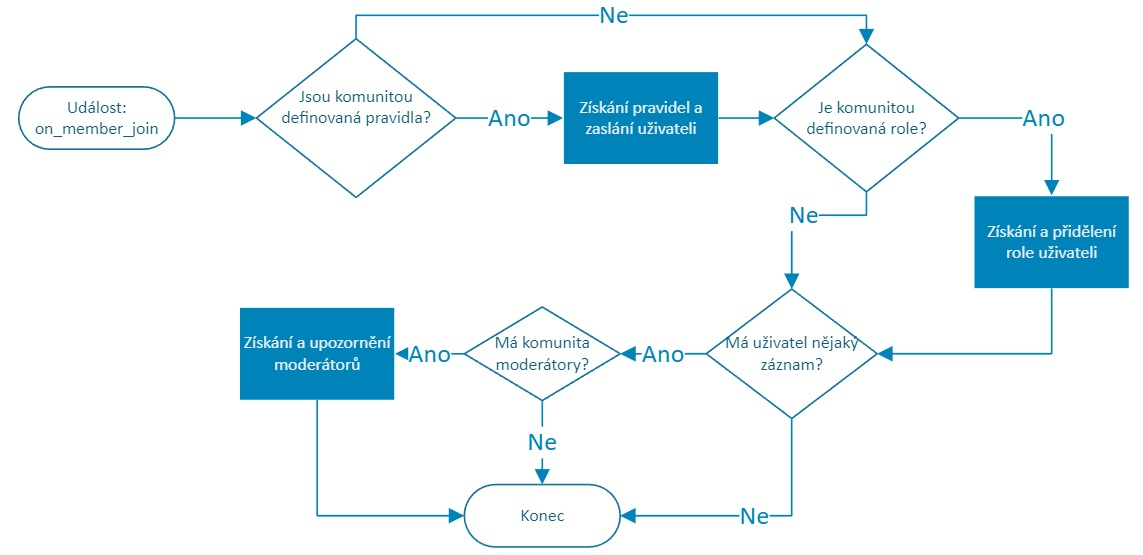
\includegraphics[scale=0.7]{on_member_join}
  \caption{\label{memberjoin}Obsloužení události při příchodu nového uživatele}
\end{figure}

\subsubsubsection{Zaslání pravidel}
Pro automatické zasílání pravidel se alespoň jedno pravidlo musí definovat na komunitním serveru
pomocí přidávacího příkazu {\it rules add}. Příkazem {\it rules reset} se smažou existující pravidla
komunity. Pro zobrazení všech platných pravidel poslouží příkaz {\it rules}. Pravidla se automaticky číslují
v pořadí ve kterém byly přidány a jsou určeny k zaslání novému uživateli po jeho připojení do soukromé zprávy.

\subsubsubsection{Přiřazení role, pravomocí}
K přiřazování role novým členům je zapotřebí, aby již na komunitním serveru přes uživatelské rozhraní
byla role nadefinována. Poté přes příkaz jako {\it autorole set} může moderátor přiřazovanou roli 
s pravomocemi nastavit.
Příkazy {\it autorole show}, {\it autorole remove} ji zobrazí nebo smažou. Takto definovaná role je 
automaticky přiřazena novému uživateli po jeho připojení na komunitní server za podmínky, že je v hierarchii 
pod rolí bota.

\subsubsubsection{Kontrola záznamů}
Kontrola záznamu se provede automaticky poté, co se uživatel, který má záznam v rejstříku, připojí na server. 
Upozornění dostanou pouze předem jmenovaní moderátoři, které lze přidat, odstranit a zobrazit příkazy 
{\it moderation add}, {\it moderation reset}, {\it moderation show}. Možnost zkontrolovat nový záznam
již stávajícího člena pomocí příkazu {\it records show}. Záznamy do rejstříku
udělají příkazy pro vyhoštění či zablokování uživatele v libovolné komunitě (i mimo stávající), kterými
jsou {\it kick} a {\it ban}.

\subsubsection{Událost: zpráva}
Zaslaný event o změně stavu, že je zaslána či upravena zpráva, bot musí zkontrolovat 
obsah zprávy a v případě závadné zprávy takovou zprávu nechat odstranit.

Následná reakce na změnu tohoto stavu obsahuje jednu činnost, zkontrolovat slovník slov a frází
v příslušném komunitním serveru nově příchozí (upravené) zprávy při jejím zpracování.
% \clearpage
\begin{figure}[h]
  \centering 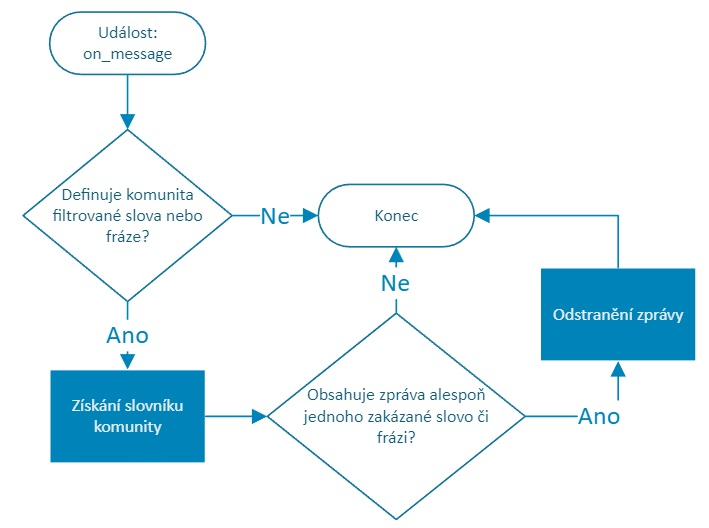
\includegraphics[scale=1]{on_message}
  \caption{\label{message}Obsloužení události nové (upravené) zprávy}
\end{figure}

Na obr. \ref{message} je vidět událost při zjištění stavu o zaslání nové zprávy, kdy se získá 
\uv{blacklist} slovník komunity a pokud ve zprávě existuje alespoň jeden výskyt ze slovníku, je taková zpráva odstraněna.
Pro událost při upravené zprávě by vypadal diagram stejně jako na obr. \ref{message}, s jediným rozdílem
a to spouštěcí událostí {\it on\_message\_edit}.

\subsubsubsection{Kontrola odeslaných a upravených zpráv}
Pro automatickou moderaci chatu botem je potřeba přes příkaz {\it filter add} definovat alespoň jedno zakázané slovo (či frázi)
v komunitním serveru. Příkazem {\it filter remove} je možné odstranit konkrétní napsané slovo či fráze, {\it filter show} zase 
zobrazí veškerý slovník. Není žádoucí, aby uživatel bez oprávnění mohl příkaz pro zobrazení spustit a nalézt případné chyby
k obcházení. Též se nerozlišuje, zda slovo či fráze má malá nebo velká písmena.

\subsection{Manuální vlastnosti}
U manuálních vlastností bota se jedná o takové akce, které pro jejich vykonání musejí být vykonány uživatelem,
tedy uživatel musí spustit příkaz přes kontextové menu obr. \ref{slash_command} lomítkového příkazu nebo 
napsáním prefixované zprávy obsahující validní název příkazu obr. \ref{prefix_command}.

Vlastnosti, které
tyto manuální příkazy mají zastat jsou pro správu uživatelů (vyhoštění, zablokování), správu událostí (vytvoření, smazání, editace),
přehrávání audio stop (přehrání, přeskočení, zobrazení fronty, úprava hlasitosti).

Tyto příkazy musejí být manuální, neboť potřebují navíc vstup od uživatele k doplnění či upřesnění
některých informací potřebných k jejich provedení.

\subsubsection{Správa uživatelů}
Pro správu uživatelů je zavedena možnost vyhostit jednoho 
či více uživatelů zároveň pomocí příkazu
{\it kick} s nepovinným odůvodněním, jejich vyhoštění vede k vytvoření záznamu v
databázi bota pro případné varování uživatelů v jiných komunitách o jejich incidentu.
Podobně na tom je příkaz zablokování {\it ban} s rozdílem, že umožňuje navíc volbu
smazání jejich výskytu v historii chatu za posledních několik předchozích dní.

Zprostředkuje
pro majitele komunity s nejvyšším oprávněním možnost zasílat hromadně všem
uživatelům jeho komunitního serveru zprávu do soukromé zprávy příkazem {\it admin
message} (či {\it embedded}), dbá se na potencionální zneužití při napadení účtu
majitele a je nastaven limit pro tuto funkcionalitu, aby nemohla být v
případě velkých komunit zneužita např. pro scam či phishing. 

Pro správu nad
hlasovými kanály má moderátor s oprávněním možnost příkazem {\it move} vybrat
\uv{mentions} připojených uživatelů a označením cílového hlasového kanálu, do
kterého je chce následně přesunout. 

\subsubsection{Správa událostí}
Zprostředkování a správa naplánovaných událostí je uděláno pomocí zapouzdřené zprávy a
interakcí příslušnými tlačítky ({\it Accept}, {\it Decline}, {\it Tentative}, {\it Cancel}).

Tlačítko accept jde použít dokud se nepřekročí nastavený limit přihlášených uživatelů, je-li
stanoven. Decline odmítne událost, tentative pro nerozhodného uživatele a tlačítko cancel
použitelné pouze pro uživatele jenž událost vytvořil pro její následné zrušení. 

Zapouzdřená zpráva umožňuje
formátovat jednotlivé položky zprávy do řad a sloupců s podporou odkazů a
obrázků. Vytvoření události se provede příkazem {\it event
echat}, který stojí za zkratkou event external chat (kvůli odlišení event internal), při jeho použití je
uživatel vyzván k doplnění informací názvu, popisku, datu, volitelnému maximálnímu počtu
přihlášených uživatelů a výběru zda bude použito číslo počtu přihlášených nebo jejich
celé jméno (vhodné pro menší událost) a místa konání buď libovolného textu či hlasového kanálu.
Pro odstranění {\it events echat} není nutné mít vlastní příkaz,
neboť stačí zprávu moderátorem odstranit.

Vedle toho existuje příkaz {\it events
ilocation} (popřípadě {\it ivoice}) pro tvorbu událostí integrovaných přímo v Discordu v
komunitě. Tyto integrované události jdou upravovat pomocí {\it events edit\_location}
({\it events edit\_voice}) a smazat příkazem {\it events\ idelete}, za pomoci vyhledání první shody hledaného názvu
události se nalezená událost odstraní.

\subsubsection{Přehrávání audio stop}
Přehrání
audio stop je zprostředkované příkazem {\it play}, který bota připojí do stejného hlasového
kanálu jako uživatel jenž příkaz vyvolal a začne přehrávat hudbu danou odkazem,
v odkazu může být pouze obsah z platformy YouTube. 

Při opakovaném použití
příkazu {\it play} se další audio zařazuje do fronty, která se dá zobrazit
příkazem {\it queue}. Pro přehrání playlistu slouží příkaz {\it play\_playlist}, který
zařadí každý přístupný obsah z playlistu do fronty. Příkaz {\it volume} umožní
upravit hlasitost přehrávaného audia a upraví hlasitost i pro další
přehrávaný obsah. Příkaz {\it pause} pozastaví přehrávání audia, příkaz {\it resume} opět
spustí přehrávání pozastaveného audia, {\it stop} zastaví audio a odpojí bota od
hlasového kanálu. Příkazy jako {\it next} přeskočí aktuálně přehrávající audio a
začne přehrávat další v pořadí, {\it shazam} určí název aktuálně přehrávané skladby.

% \subsection{Výběr hostingu}

\newpage
\section{Implementace}
Tato kapitola se zaobírá, jakým způsobem je bot vyvinut a implementován. 

Pro implementaci
bota byla zvolena knihovna {\it discord.py}, která zajistí komunikaci bota s Discord API, knihovna
{\it yt\_dlp}, která umožní komunikovat s platformou YouTube a nepřímo použitá knihovna pro manipulaci s audiem {\it FFmpeg}. 
Knihovna {\it asyncio} umožňuje kód spouštět a vykonávat asynchronně. Jako další knihovny jsou použity 
{\it aiohttp} pro potřeby komunikace s REST API, {\it aiofiles} pro asynchronní přístup k souborům a knihovna {\it python-dotenv}
sloužící jen pro uložení autorizačního tokenu mimo zdrojový kód za účelem bezpečnosti.

Je také implementována vlastní databáze za pomocí \acrshort{json} formátu, neboť není nutné ukládat
velké množství dat a vedle aplikace bota mít databázový systém by bylo paměťově náročnější než samotná aplikace bota.

\subsection{Souborová struktura}

\begin{figure}[h]
  \centering 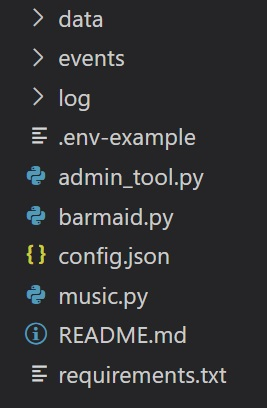
\includegraphics[scale=1]{filesystem}
  \caption{\label{files}Souborový systém aplikace bota}
\end{figure}

Na obr. \ref{files} je souborová struktura rozdělena následujícím způsobem:

\begin{description}
  \item[\texttt{data}] \hfill \\
  Složka obsahuje veškerou práci s daty se kterými bot nakládá, jako je 
  načtení informací z konfiguračního souboru, hlavní databáze bota a databáze 
  záznamů uživatelů, modul pro komunikaci nad zmíněnými databázemi.

  \item[\texttt{events}] \hfill \\
  Složka obsahuje moduly související s plánovanými událostmi.

  \item[\texttt{log}] \hfill \\
  Složka obsahuje modul pro vytvoření a obsluhu logů jenž bot využívá a soubor, do kterého
  se log zapisuje.

  \item[\texttt{.env-example}] \hfill \\
  V souboru .env-example se nachází placeholder pro autorizační token bota, který je potřeba
  doplnit při zprovoznění vlastního účtu bota. Soubor je poté nutné přejmenovat jako .env a ponechat.

  \item[\texttt{admin\_tool.py}] \hfill \\
  Je modul obsahující všechny příkazy týkající se správy komunity, uživatelů.

  \item[\texttt{barmaid.py}] \hfill \\
  Je hlavní spouštěcí soubor bota, který připojí ostatní moduly a bota přihlásí do Discordu.
  Definuje také chování některých eventů websocketu, kterým bot naslouchá a obsluhuje je.

  \item[\texttt{config.json}] \hfill \\
  Je základní konfigurační soubor ve kterém se v případě vlastního bota musí 
  vhodně nastavit údaje s identifikátorem bota, dále zde lze upravovat chování bota
  k příkazům.

  \item[\texttt{music.py}] \hfill \\
  Je modul obsahující všechny příkazy týkající se přehrávání audia.

  \item[\texttt{README.md}] \hfill \\
  Je soubor obsahující popis projektu a jeho instalaci, určený pro repozitář na Github platformu.

  \item[\texttt{requirements.txt}] \hfill \\
  Je soubor obsahující popis všech potřebných knihoven v příslušných verzích pro
  instalaci skrze {\it Python Installer Package}, zkráceně {\it pip}.

\end{description}

\subsection{Spouštěcí soubor}
Jako hlavní spouštěcí soubor je modul s názvem {\it barmaid.py}, který 
při spuštění interpretem připojí ostatní moduly, nastaví eventy na které bot bude reagovat z websocketu,
připojí se k Discordu, bota autorizuje a spustí, spouštěcí modul rovněž definuje funkci pro správný
chod prefixových příkazů.

\begin{kicode}{python}{intents}{Nastavení oprávnění bota v Discord API}[h!]
  # Intents manages some level of permissions bot can do
  INTENTS = Intents.default()
  INTENTS.members, INTENTS.presences = True, True
  INTENTS.message_content, INTENTS.reactions = True, True
\end{kicode}

Ve zdrojovém kódu \ref{intents} definujeme botu přístup ke členům komunitního serveru a jejich aktivit,
obsahu zpráv a jejich reakcí.

\begin{kicode}{python}{prefix}{Funkce určující prefix}[h!]
  async def get_prefix(client:commands.Bot, message:Message):
    if not message.guild:
        return commands.when_mentioned_or(S.DEFAULT_SERVER_PREFIX)(client, message)
    
    prefix = await read_db(DATABASE, message.guild.id, 'prefix')
    if not prefix:
        is_okay = await insert_db(DATABASE, message.guild.id, 'prefix', S.DEFAULT_SERVER_PREFIX)
        if not is_okay:
            return
        prefix = S.DEFAULT_SERVER_PREFIX
    return commands.when_mentioned_or(prefix)(client, message)
\end{kicode}

Zdrojový kód \ref{prefix} je funkce, která zajistí zjištění příslušného prefixu používaného
v konkrétním komunitním serveru je-li nastaven, jinak se použije symbol \uv{.} jako výchozí.

\begin{kicode}{python}{botc}{Vytvoření bota}[h!]
  # Client is top level var because of @ decorator for events
  CLIENT = commands.Bot(command_prefix=get_prefix, intents=INTENTS)
  
  # Create of log handle
  log_handle:logging.Logger = setup_logging()
\end{kicode}

Kód \ref{botc} zajišťuje vytvoření instance třídy {\it commands.Bot} za použití 
prefixové funkce a oprávnění, které bot bude mít definované z předchozích zdrojových kódů \ref{intents} a \ref{prefix}.
Také vytváří proměnnou {\it log\_handle}, pomocí které lze zapisovat log při běhu aplikace.

\begin{kicode}{python}{webevent}{Ukázka callback funkce websocket eventu}[h!]
  @CLIENT.event
  async def on_command_error(ctx:Context, error:commands.CommandError):
      if isinstance(error, commands.CommandNotFound):
          await ctx.send(error, ephemeral=True)
          return
\end{kicode}

Kód \ref{webevent} definuje callback funkci, která bude reagovat na události z websocketu, pro
ukázku je zde uvedena pouze jedna, ale spouštěcí soubor obsahuje těchto funkcí více:
{\it on\_ready}, {\it on\_guild\_join}, {\it on\_member\_join}, {\it on\_message}, {\it on\_message\_edit}, 
{\it on\_message\_error}. Tyto funkce budou ještě popsány v implementaci dále.

Zdrojový kód \ref{start} spustí bota pomocí autorizačního tokenu, který nalezne v 
souboru {\it .env} a následně spustí funkci \ref{extensions} pro načtení
ostatních modulů do instance třídy bota v proměnné {\it CLIENT}. Kód \ref{slashcommands} 
je spuštěn poté co je bot úspěšně nastartován a dorazí jeden z prvních eventů websocketu
k synchronizaci lomítkových příkazů, slouží k tomu funkce {\it setup\_hook}. Zároveň s tím
nastavuje třídu {\it EventView}, o té ještě později, jako persistentní vůči restartu, aby tlačítka
jenž bot vytváří fungovali i po jeho vypnutí a následném zapnutí.

\begin{kicode}{python}{slashcommands}{Synchronizace příkazů}[h!]
  @CLIENT.event
  async def setup_hook():
      synced_commands =  await CLIENT.tree.sync()
      print(f"In-app commands have been synchronized.")
      CLIENT.add_view(EventView())
\end{kicode}

\begin{kicode}{python}{extensions}{Instalace modulů}[h!]
  # Listed modules to be loaded
  EXTENSIONS = [
      "admin_tool",
      "events.event",
      "music",
  ]

  async def install_extensions(target:commands.Bot):
    for ext in EXTENSIONS:
        await target.load_extension(ext)
\end{kicode}

\begin{kicode}{python}{start}{Spuštění bota}[h!]
  if __name__ == "__main__":
    load_dotenv()
    CONNECTION_TOKEN = os.getenv("TOKEN")
    
    loop = asyncio.new_event_loop()
    
    loop.run_until_complete(install_extensions(CLIENT))
    CLIENT.run(CONNECTION_TOKEN)
\end{kicode}

\subsection{Vytvoření aplikace a účtu jako bot}
Vytvoření aplikace probíhá po přihlášení hlavním účtem uživatele na webové stránce platformy a navštívením webové adresy {\it discord.com/developers/applications}, 
zde je v pravém horním rohu tlačítko \uv{Create Application} a vyzvání k výběru jména aplikace viz obr. \ref{create}, toto jméno bude jménem účtu bota.

\begin{figure}[h]
  \centering 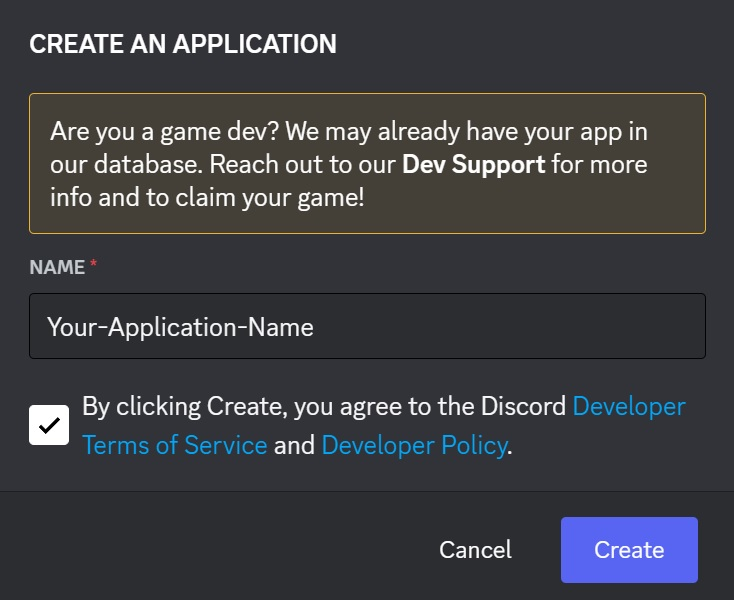
\includegraphics[scale=1]{create}
  \caption{\label{create}Vytvoření aplikace}
\end{figure}

Po vytvoření aplikace je nutné přejít do sekce \uv{Bot} a vytvořit nového bota tlačítkem \uv{Add Bot} 
viz obr. \ref{bot}.

\begin{figure}[h]
  \centering 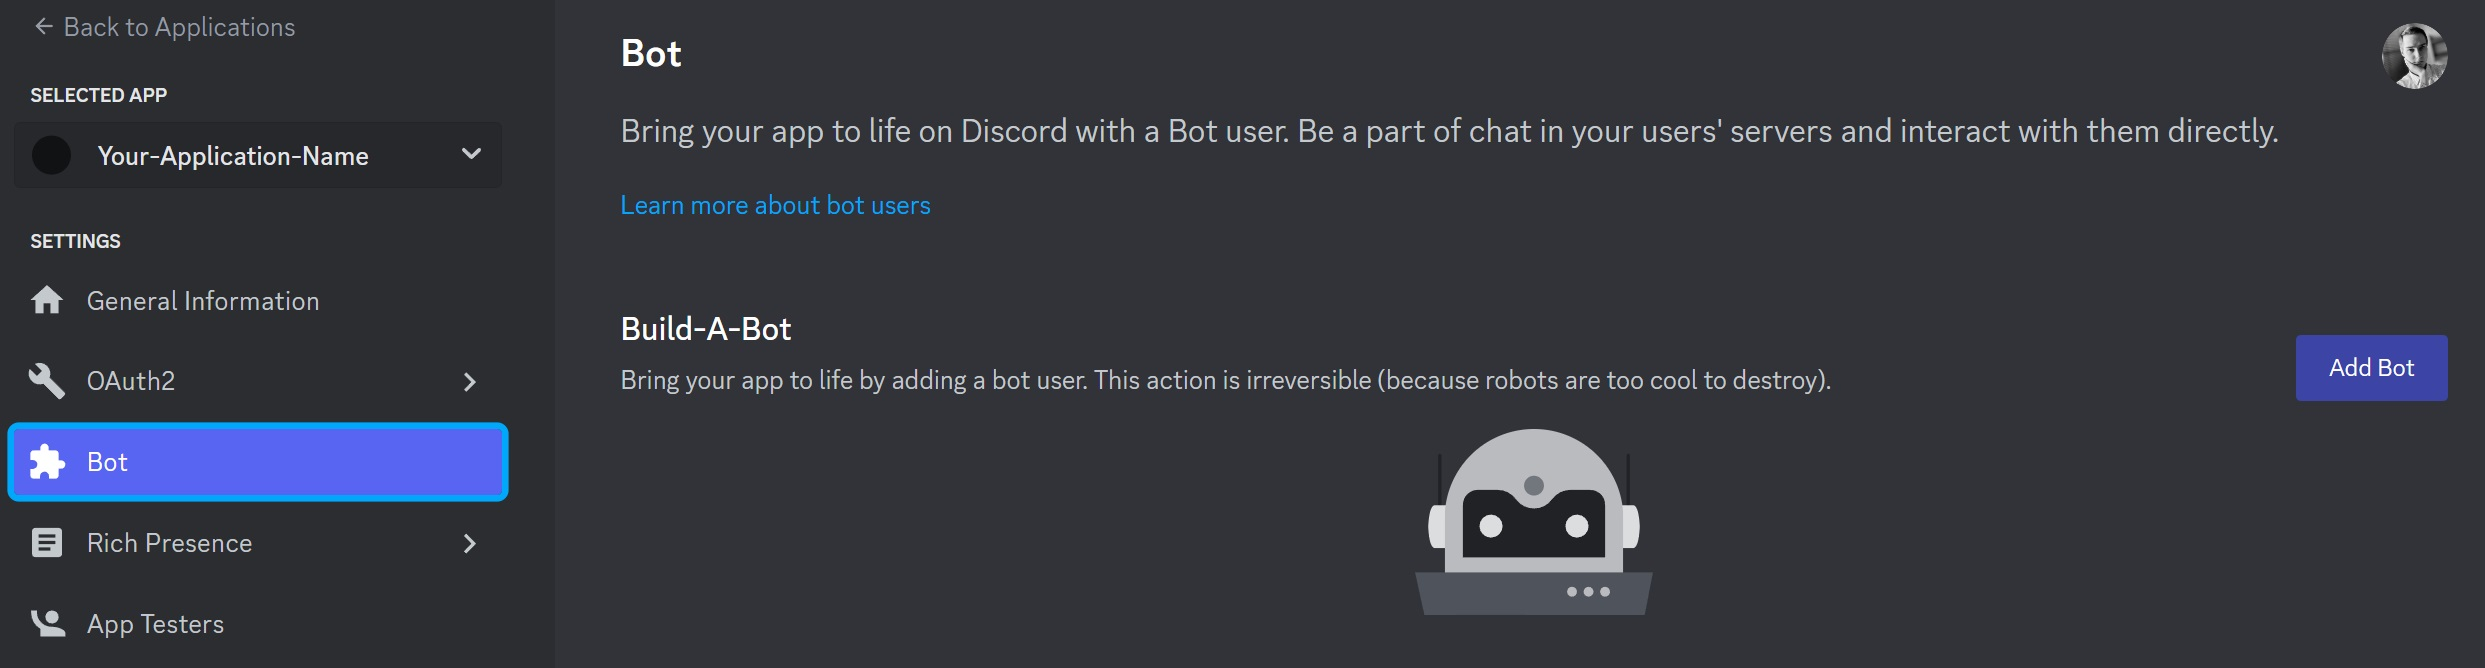
\includegraphics[scale=0.32]{bot}
  \caption{\label{bot}Vytvoření aplikace jako bot}
\end{figure}

Po vytvoření bota se zpřístupní účet bota a je možné zobrazit jeho autorizační token
jednorázovým tlačítkem \uv{View Token} viz obr. \ref{token}. Tento token 
slouží ke spuštění bota hlavním spouštěcím souborem, token je nutné vložit do souboru
{\it .env-example}
na příslušné místo a přejmenovat soubor na {\it .env}.

\begin{figure}[h]
  \centering 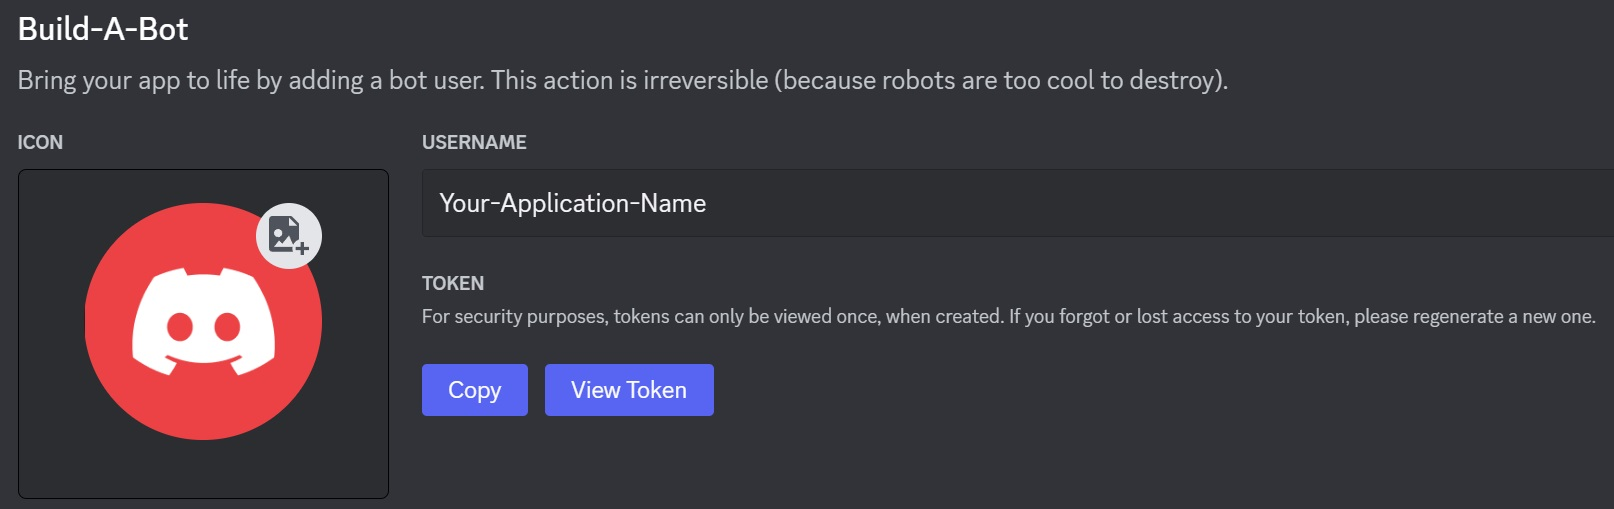
\includegraphics[scale=0.5]{token}
  \caption{\label{token}Získání autorizačního tokenu bota}
\end{figure}

\begin{figure}[h]
  \centering 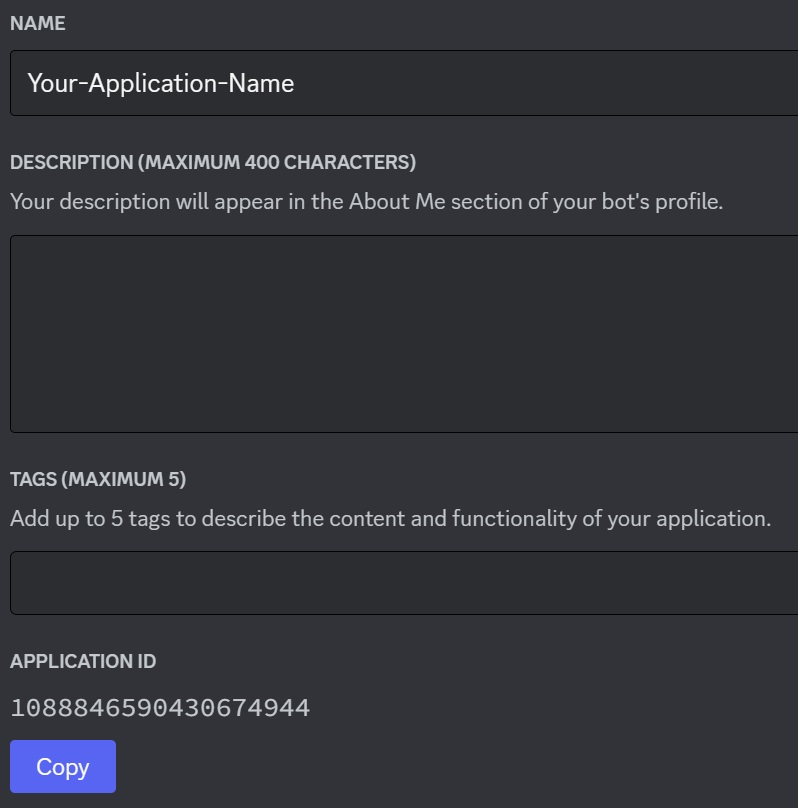
\includegraphics[scale=0.6]{appid}
  \caption{\label{appid}Identifikátor aplikace}
\end{figure}

V sekci \uv{General Information} na webové stránce lze, viz obr. \ref{appid},
nalézt {\it application id}, kterým je nutné příslušně vyplnit soubor {\it config.json}.

\subsection{Ukládání dat}
Ukládání informací je nutné, aby bot mohl rozlišovat data týkající se pouze konkrétního
komunitního serveru. Ukládá tedy pro každý komunitní server jeho prefix, pravidla, roli pro přidělení
a veškerou organizaci naplánovaných událostí. Dále používá globální databázi pro záznamy
uživatelů, jenž byly z některého serveru vyhoštěni či z nějakého důvodu zablokovaní.

Pro dva nezávislé soubory s daty {\it user\_records.json} a {\it data.json} je zaveden 
univerzální přístup modulem {\it jsonified\_database.py}, který umožňuje čtení a zápis
do těchto souborů na základě výběru.

K otevření cíleného souboru slouží kód \ref{open}, který zajišťuje asynchronní
přístup k souboru a vrátí jeho celý obsah ve formátu \acrshort{json}.
% \clearpage

\begin{kicode}{python}{open}{Otevření databázového souboru}[h!]
  async def open_file(file_name:str) -> dict:
    async with aiofiles.open(file_name, READ_FLAG) as f:
        contents = await f.read()
        json_as_dict = json.loads(contents)
    return json_as_dict
\end{kicode}

\newpage
Pro zápis do cíleného souboru slouží funkce {\it flush\_file} ze zdrojového kódu \ref{flash}, který
zajišťuje asynchronní přístup k souboru a zapisování do něj.

\begin{kicode}{python}{flash}{Zápis do databázového souboru}[h!]
  async def flush_file(file_name:str, data:dict) -> str:
      async with aiofiles.open(file_name, WRITE_FLAG) as f:
          await f.write(data)
      return data
\end{kicode}

Za pomocí těchto dvou základních univerzálních funkcí jako je čtení a zápis jde dále
vytvořit funkci, která přečte danou hodnotu podle klíče v databázi, slouží k tomu funkce
{\it read\_db} viz zdrojový kód \ref{read}.

\begin{kicode}{python}{read}{Čtení v databázovém souboru}[h!]
  async def read_db(file_name:str, id:int, key:str): 
    id_str = str(id)
    data = await open_file(file_name)

    try:
        value_by_key = data[id_str][key]
        return value_by_key
    except KeyError as e:
        return None
\end{kicode}

Základní funkcí aktualizace dat v databázových souborech slouží funkce {\it update\_db} viz zdrojový
kód \ref{update}, dále modul {\it jsonified\_database.py} obsahuje i další funkce jako {\it insert\_db},
{\it delete\_from\_db}, {\it add\_id} a {\it id\_lookup}.
\newpage

\begin{kicode}{python}{update}{Aktualizace dat v databázovém souboru}[h!]
  async def update_db(file_name:str, id:int, key:str, new_value):
    id_str = str(id)
    data = await open_file(file_name)

    try:
        data[id_str][key] = new_value
    except KeyError:
        return None
    
    new_data = json.dumps(data, indent=2)
    result = await flush_file(file_name, new_data)
    return result
\end{kicode}

% \subsection{Spouštění příkazů}
\subsection{Struktura příkazů v kódu}
Struktura příkazu je demonstrována a detailněji popsána na příkladu jednoho z příkazů.
V kódu \ref{clear_command} je vidět struktura v kódu. Řádek č. 1 určuje pomocí
dekorátoru o jaký příkaz se jedná, {\it @commands.command()} definuje prefixovaný příkaz, {\it 
@commands.hybrid\_command(with\_app\_invoke=True)} definuje prefixový příkaz a k němu stejnojmenný 
lomítkový příkaz na základě pravdivostní hodnoty argumentu 
% {\it with\_app\_invoke}
, {\it @commands.hybrid\_group()} pak 
podobně jako {\it hybrid\_command} definuje hlavní příkaz a k němu podpříkazy, lze později vidět v implementaci
plánovaných událostí v podkapitole. Ve stejném dekorátoru lze definovat jméno příkazu, není-li definováno
pak je použito jako jméno název definované funkce na řádku č. 6, a případné \uv{aliasy} pouze pro
prefixované příkazy.

% \begin{figure}[h]
%   \centering 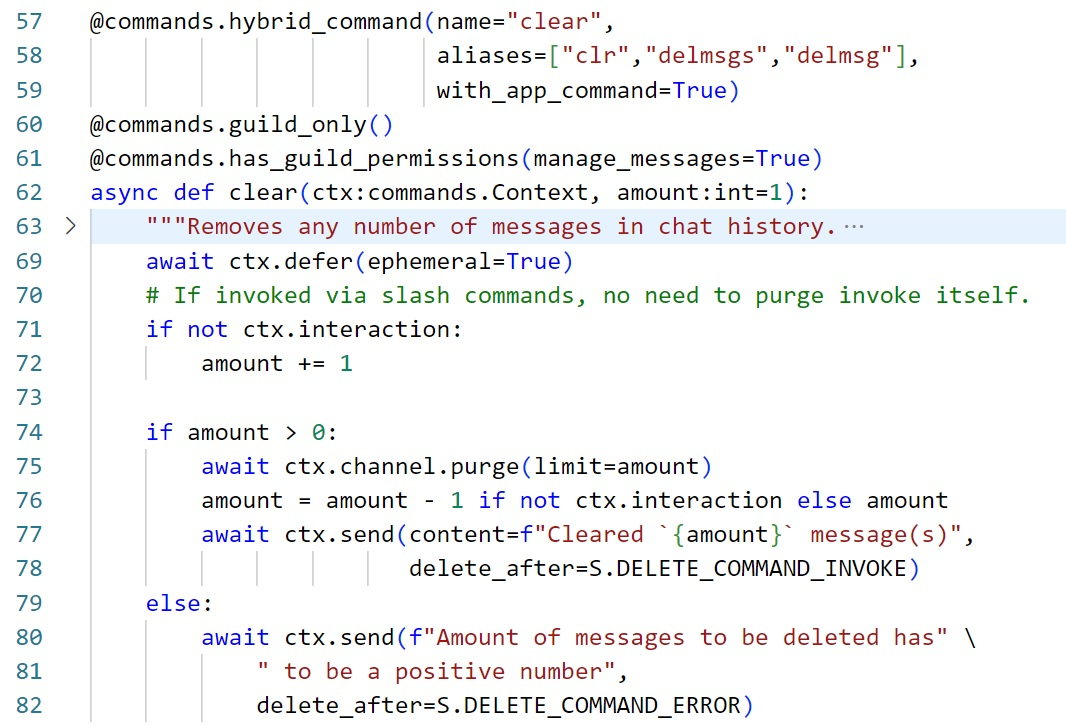
\includegraphics[scale=0.8]{codestructure}
%   \caption{\label{codes}Ukázka struktury příkazu v kódu, příkaz {\it clear}}
% \end{figure}

\begin{kicode}{python}{clear_command}{Ukázka struktury příkazu v kódu, příkaz {\it clear}}[h!]
  @commands.hybrid_command(name="clear",
    aliases=["clr","delmsgs","delmsg"],
    with_app_command=True)
  @commands.guild_only()
  @commands.has_guild_permissions(manage_messages=True)
  async def clear(ctx:commands.Context, amount:int=1):
    """Removes any number of messages in chat history.

    Args:
        ctx: Current context of the message that invoked the command.
        amount (optional): Number of messages to delete.
    """
    # If invoked via slash commands, no need to purge call itself.
    await ctx.defer(ephemeral=True)    
    if not ctx.interaction:
      amount += 1

    if amount > 0:
      await ctx.channel.purge(limit=amount)
      amount = amount - 1 if not ctx.interaction else amount
      await ctx.send(content=f"Cleared `{amount}` message(s)")
    else:
      await ctx.send(f"Amount of messages to be deleted has" \
                      " to be a positive number")
\end{kicode}

Řádek č. 4 určuje rozsah platnosti příkazu, dekorátor {\it @commands.guild\_only()} určí příkaz
pouze pro použití uvnitř komunitního serveru, není-li definováno pak příkaz je platný i ve soukromé zprávě
s botem.

Dekorátor {\it @commands.has\_guild\_permissions()} na řádku č. 5 ověřuje, zda uživatel
jenž příkaz vyvolal má dostatečná oprávnění, pokud nemá je programem vyvolána výjimka, která může být buď
obsloužena pomocnou funkcí se stejnojmenným dekorátorem jako je název příkazu a vlastností error. Pro
tuto funkci {\it clear} by to bylo například {\it @clear.error} a funkce s libovolným jménem např. {\it clear\_error}, pro
příklad jak taková chybová funkce může vypadat viz. zdrojový kód \ref{clearerror}. Není-li taková funkce definována, je pak odchycena
eventem websocketu s názvem {\it on\_command\_error}.

Řádek č. 6 definuje funkci, která se vykoná při zavolání příkazu za pomoci prefixu/lomítka dle příslušného
dekorátoru u funkce, funkce musí mít vždy jeden argument {\it ctx} třídy {\it commands.Context}, který 
obsahuje všechny informace z cache bota a lze pomocí tohoto objektu zjistit autora příkazu, komunitní server
a na základě toho rozlišovat chování příkazu. Zbytek argumentů je na vývojáři daného příkazu. Při použití 
statického typování pak u lomítkových příkazů dochází ke správné nápovědě, co může do argumentu vstupovat. Je-li uvedena výchozí hodnota argumentu
pak se tento argument stává nepovinným pro příkaz.

Zabalené řádky č. 7-12 obsahují dokumentaci funkce, jenž je
pak násladně použita pro popisky příkazů a jejich argumentů, je-li příkaz volán jako lomítkový.

První řádek v těle funkce č. 14 slouží k obsloužení příkazu hybridně, buď interakcí skrze lomítkový příkaz
nebo prefixovanou zprávu. Pokud se jedná o lomítkový příkaz, je nutné odpovědět pomocí {\it ctx.send()} do deseti vteřin. 
Trval by výpočet déle, pak vyprší timeout interakce a {\it ctx.send()} vyvolá výjímku, tento řádek zvýší
timeout interakce z deseti vteřin na 15 minut. Pokud příkaz byl vyvolaný pomocí prefixové zprávy, pak tento kód řádku č. 14
nemá žádný efekt a neprovádí nic s navýšením timeoutu. Pouze v obou případech může definovat skrze {\it ephemeral=True} viditelnost
odpovědi pouze autorovi, co příkaz vyvolal.

Řádky č. 15 až 24 obsahují zbytek těla funkce a chování celého příkazu, v tomto příkladu 
smazání určitého počtu zpráv v textovém kanále, jenž byl příkaz spuštěn.

% \begin{figure}[h]
%   \centering 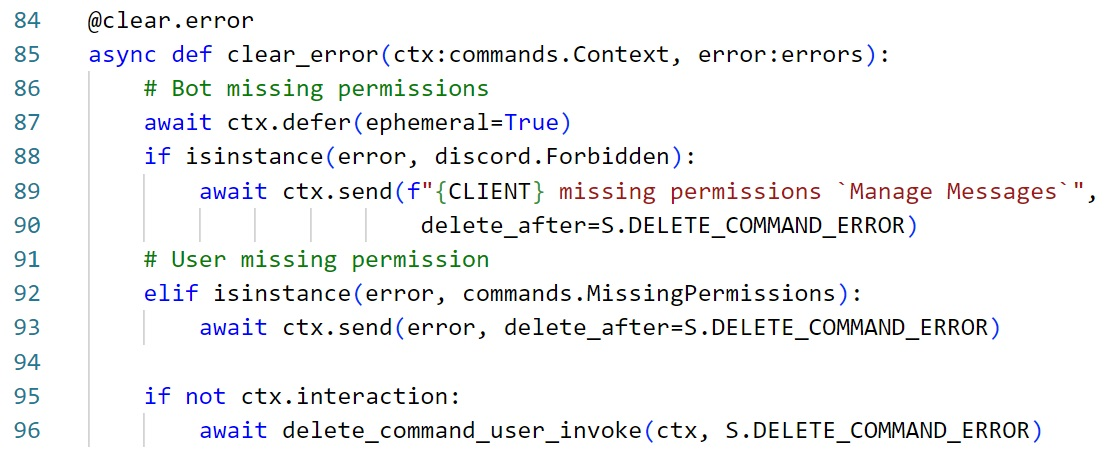
\includegraphics[scale=0.8]{clearerror}
%   \caption{\label{clearerror}Chybová funkce k příkazu {\it clear}}
% \end{figure}

\begin{kicode}{python}{clearerror}{Chybová funkce k příkazu {\it clear}}[h!]
  @clear.error
  async def clear_error(ctx:commands.Context, error:errors):
      # Bot missing permissions
      await ctx.defer(ephemeral=True)
      if isinstance(error, discord.Forbidden):
          await ctx.send(f"{CLIENT} missing permissions `Manage Messages`",
                          delete_after=S.DELETE_COMMAND_ERROR)
      # User missing permission
      elif isinstance(error, commands.MissingPermissions):
          await ctx.send(error, delete_after=S.DELETE_COMMAND_ERROR)
      
      if not ctx.interaction:
          await delete_command_user_invoke(ctx, S.DELETE_COMMAND_ERROR)
\end{kicode}

\newpage
\subsection{Pravidla komunit}
Pravidla komunit spadají pod správu a nacházejí se v modulu {\it admin\_tool.py}. Zde
existují příkazy {\it rules} pro zobrazení pravidel, {\it addrule} pro přidání nového pravidla
ke stávajícím, {\it delrule} pro smazání konkrétního pravidla, {\it rules\_reset} pro odstranění
všech platných pravidel.

\begin{figure}[h!]
  \centering 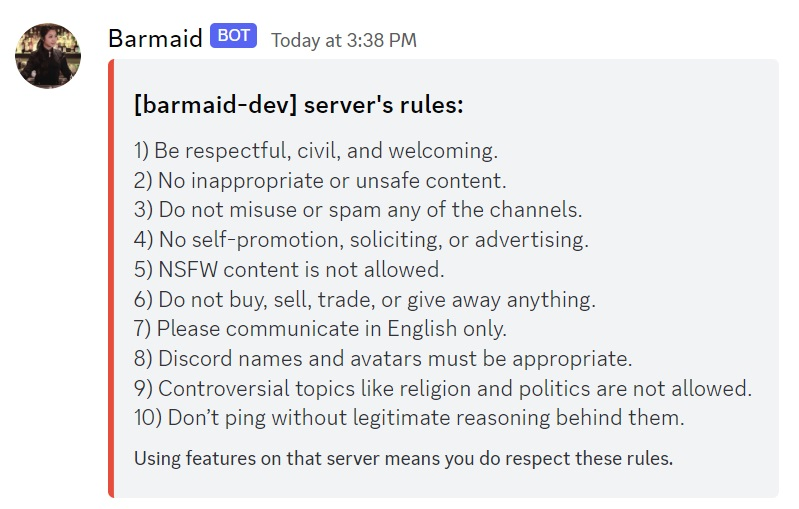
\includegraphics[scale=0.9]{barmaid_rules2}
  \caption{\label{barmaid_rules}Ukázka zaslaných pravidel novým členům}
\end{figure}

Pro zprovoznění automatického zasílání pravidel botem musí existovat
alespoň jedno pravidlo zadané uživatelem s potřebnými moderátorskými pravomocemi. Pokud role uživatele nesplňuje
příslušná oprávnění, jsou mu některé z těchto příkazů nepovoleny a pouze napíší, které pravomoce jsou potřeba
k jejich spuštění. K automatickému zaslání slouží callback funkce {\it on\_member\_join} reagující na event
websocketu v hlavním spouštěcím souboru {\it barmaid.py}, tuto callback funkci také lze vidět ještě v kapitole
týkající se kontroly uživatelů. Zde je uvedena pouze její část, týkající se pravidel, tedy přenechání na funkci {\it send\_guild\_rules}.

\begin{kicode}{python}{memberjoin}{Event (websocket) připojený člen}[h!]
  @CLIENT.event
  async def on_member_join(member:Member):
      # ... get role id from database and find corresponding role
      await member.add_roles(role_to_give)
      
      await send_guild_rules(member, member.guild)

      if await check_records(member):
          await aware_of_records(member, member.guild)
\end{kicode}

\begin{kicode}{python}{grules}{Zaslání pravidel komunity}[h!]
  async def send_guild_rules(member:Member, guild_joined:Guild):
      # ... get rules from database, format them
      emb = Embed(title=f"[{guild_joined.name}] server's rules:",
                  description=formated_output,
                  color=Colour.red())
      emb.set_footer(text="Being part of that server means you do respect these rules.")
      await member.send(embed=emb)
\end{kicode}

Event websocketu {\it on\_member\_join} popsaný callback funkcí \ref{memberjoin}
je spuštěn při připojení nového člena do serveru a funkce přiděluje pravomoce, o tom v pozdější kapitole. Přenechává
na funkci {\it send\_guild\_rules} zaslání připojenému členovi příslušná pravidla serveru. Nejsou-li stanovena žádná
pravidla předem, není zasláno nic.

Funkce \ref{grules} obstarává zaslání uživateli, který se připojil, příslušná pravidla serveru, která se pokusí nalézt
v databázi, naformátuje jejich výstup a zapouzdří je do zprávy, kterou mu následně zašle do soukromého chatu.

Zdrojový kód \ref{rules} slouží k zobrazení pravidel příslušné komunity, pravidla získává z 
databáze bota a formátuje každá pravidlo na vlastní řádek s řadovou číslovkou. Pokud žádná
pravidla ještě neexistují, informuje o tom chybovou hláškou, taktéž odstraní prefixovou zprávu pokud ta
příkaz vyvolala.

\begin{kicode}{python}{rules}{Zobrazení pravidel}[h!]
  @commands.hybrid_command(with_app_command=True)
  @commands.guild_only()
  async def rules(ctx:commands.Context):
      # ... handle slash command or prefix invoke, permissions
          
      # ... find rules, format them
      if guild_rules:
          await ctx.send(formated_output,
                          delete_after=S.DELETE_MINUTE)
          return
      await ctx.send("No rules have been set yet.",
                     delete_after=S.DELETE_COMMAND_INVOKE)
\end{kicode}

\begin{kicode}{python}{addrule}{Přidání pravidla}[h!]
  @commands.hybrid_command(with_app_command=True)
  @commands.guild_only()
  async def addrule(ctx:commands.Context, *, new_rule:str):
      # ... handle slash command or prefix invoke, permissions
      
      # ... check database for already existing rules, if so
      # then appends new to them
      
      updated = await update_db(DATABASE,
                     ctx.guild.id, "guild-rules", rules)
      if updated:
          await ctx.send("New rule applied.")
          return
      await database_fail(ctx)
\end{kicode}

\newpage
K přidání nového pravidla slouží zdrojový kód \ref{addrule}, který nejdříve zkontroluje dostatečná
oprávnění uživatele, získá stávající pravidla a k nim připojí pravidlo nové. Poté aktualizuje
záznam v databázi a oznamí úspěšné zaznamenání pravidla. Pokud něco selže, je o tom uživatel 
informován chybovou hláškou. Pokud byla k vyvolání příkazu použita prefixová zpráva, bude odstraněna.


O vyresetování všech pravidel se postará zdrojový kód \ref{resetrules}, který zkontroluje potřebné pravomoce,
odstraní prefixovanou zprávu jenž příkaz vyvolala (pokud byla použita), odstraní záznam z databáze a informuje o úspěšném či neúspěšném vykonání.

\begin{kicode}{python}{resetrules}{Resetování pravidel}[h!]
  @commands.hybrid_command(with_app_command=True, 
                        name="reset-rules")
  @commands.guild_only()
  async def rules_reset(ctx:commands.Context):
      # ... handle slash command or prefix invoke, permissions
      
      reset = await delete_from_db(DATABASE, 
                     ctx.guild.id, "guild-rules")
      if reset:
          await ctx.send("Rules no longer apply.", 
                          delete_after=S.DELETE_COMMAND_INVOKE)
          return
      await database_fail(ctx)
\end{kicode}

\newpage
Zdrojový kód \ref{delrule} smaže pravidlo na příslušném indexu, příkaz zkontroluje potřebné pravomoce uživatele
jenž příkaz vyvolal. Pokud byla použita prefixová zpráva k jejímu vyvolání dojde k jejímu smazání, odstraní se konkrétní pravidlo
na daném indexu v databázi a dojde k informování uživatele o provedení, ať úspěšném nebo neúspěšném.

\begin{kicode}{python}{delrule}{Smazání pravidla}[h!]
  @commands.hybrid_command(with_app_command=True)
  @commands.guild_only()
  async def delrule(ctx:commands.Context, index:int):
      # ... handle slash command or prefix invoke, permissions

      # ... find rules in database
      if not guild_rules:
          await ctx.send("There are no rules therefore nothing to delete.")
          return
      del guild_rules[str(index-1)]
      idx = 0
      new_dict = {}
      for _, value in guild_rules.items():
          new_dict[str(idx)] = value
          idx += 1
  
      # ... update database
\end{kicode}


\subsection{Kontrola zpráv}
O kontrolu zpráv se stará hlavní spouštěcí modul, neboť v něm jsou definované všechny websocket eventy, na které bot reaguje 
a naslouchání zprávám je také event.
Jako eventy pro kontrolu zpráv slouží {\it on\_message} a {\it on\_message\_edit}, kde v těle těchto callback
funkcí je zavolána funkce {\it check\_blacklist}, která se stará o zkontrolování zablokovaných slov v příslušné komunitě a dojde-li ke
shodě je příslušná zpráva odstraněna. Z modulu ke správě {\it admin\_tool.py} pomáhají k definování zakázaných slov
příkazy {\it filter show}, {\it filter add}, {\it filter remove} pro zobrazení všech zablokovaných slov nebo frází, přidání/odebrání nového slova či fráze.

Ve zdrojovém kódu \ref{onmessage}  dojde i ke kontrole vlastní zprávy zaslané botem, tuto skutečnost bot ignoruje a má pro sebe
výjimku. Dochází ke kontrole, zda zpráva byla poslaná v komunitním serveru. Pokud ano předává se zpráva ke kontrole příslušnému serveru
funkcí {\it check\_blacklist} viz kód \ref{blacklist}, dále posílá zprávu ke zpracování prefix příkazů, které se mohou potencionálně
ve zprávě nacházet. V neposlední řadě informuje uživatele, že bot nebude reagovat na interakce skrze soukromý chat s botem.

\begin{kicode}{python}{onmessage}{Event (websocket) nové zprávy}[h!]
  @CLIENT.event    
  async def on_message(msg:Message):
      if msg.author == CLIENT.user:
          return
      if msg.guild:
          await check_blacklist(msg.guild, msg)
          await CLIENT.process_commands(msg)
          return
      await msg.channel.send("I don't serve any drinks here.")
\end{kicode}

Kód \ref{blacklist} provádí smazání zprávy pokud zpráva obsahuje alespoň jedno slovo či frázi definovanou příslušnou
komunitou jako nevhodnou, bot dává výjimku skrze {\it is\_blacklist\_exception} funkci pouze takové zprávě, která je zamýšlena
k použití při odstraňování zablokovaného slova či fráze neboť tato zpráva bude takové slovo/frázi obsahovat.

\begin{kicode}{python}{blacklist}{Kontrola obsahu zprávy}[h!]
  async def check_blacklist(guild:Guild, msg:Message):
    if await is_blacklist_exception(msg):
        return
    
    # ... finds blacklist in the database
    
    for w in blacklist:
        if w in msg.content:
            await msg.delete()
            await msg.author.send(f"Word \"{w}\" is restricted to use in `{guild.name}`")
\end{kicode}

Aby nebylo možné napsat nežádoucí slova \uv{na podruhé} obcházením funkcionality úpravy zpráv, tak je potřeba kontrolovat 
nežádoucí obsah i v nich, od toho slouží zdrojový kód \ref{onedit}, který je zjednodušenou verzí kódu při zaslání první zprávy
{\it on\_message} \ref{onmessage}. 

\begin{kicode}{python}{onedit}{Event (websocket) upravené zprávy}[h!]
  @CLIENT.event
  async def on_message_edit(before:Message, after:Message):
      if after.author == CLIENT.user:
          return
      if after.guild:
          await check_blacklist(after.guild, after)
\end{kicode}

\newpage
\subsection{Kontrola uživatelů, přidělení pravomocí}
Kontrola uživatelů je zajištěna pomocí eventu websocketu {\it on\_member\_join} 
v hlavním spouštěcím souboru {\it barmaid.py}. Pro nastavení této funkcionality slouží příkazy
z modulu {\it admin\_tool.py} k nastavení moderátorů komunity a příkaz pro zobrazení záznamu 
konkrétního uživatele. Souvisejícími příkazy s touto funkcionalitou jsou {\it moderation show}, 
{\it moderation add}, {\it moderation reset}, {\it records}.

V předchozí kapitole již byl zmíněn zdrojový kód \ref{memberjoin}, kde je 
vysvětlena jedna část funkcionality týkající se pravidel, nyní je vysvětlena druhá část týkající se
následné kontroly připojeného uživatele a přidělení pravomocí.

Zmíněný zdrojový kód obsahuje funkci {\it check\_records}, která zkontroluje, zda uživatel má
záznam v databázi. Pokud má je zavolána funkce {\it aware\_of\_records}, která zajistí zaslání
informace všem moderátorům příslušné komunity o existenci záznamů nového člena.

Kód \ref{checkrecord} vrací pravdivostní hodnotu, zda uživatel má záznam v databázi, 
záznam má v databázi pouze pokud je u něho evidován alespoň jeden z prohřešků.

\begin{kicode}{python}{checkrecord}{Zjištění existence záznamu uživatele}[h!]
  async def check_records(member:Member)->bool:
    # ... gets records of member from database
    if records:
        return True
    return False
\end{kicode}

Zdrojový kód funkce \ref{awarerecords} se postará o zjištění a nalezení definovaných moderátorů komunity
a jejich následné upozornění a sdělení o celkovém počtu evidovaných prohřešků uživatele, odkáže je jiný příkaz
pomocí kterého si mohou detailněji prohlédnout o jaké prohřešky se jedná.

\begin{kicode}{python}{awarerecords}{Oznámení o existenci záznamů nového uživatele}[h!]
  async def aware_of_records(member:Member, guild:Guild):
    # ... gets corresponding moderators
    # and all records of the member from database
    
    for m in mods:
        await m.send(f"{member} joined {guild.name} with `{len(bad_records)}` " +
              "bad records.\nUse `/records @mention` on your server " +
              "to see more information.")
\end{kicode}

\newpage
Zdrojový kód \ref{memberjoin} obsahuje ještě třetí funkcionalitu, přidělení role s pravomocemi novému členu,
o které se nestará vlastní definovaná funkce, ale pouze nalezení definované role pro přidělení v komunitě a přidělením
skrze metodu {\it add\_roles()} třídy {\it discord.Member} z {\it discord.py} knihovny. Souvisejícími příkazy pro definování
takové role k přidělení jsou: {\it autorole show}, {\it autorole set}, {\it autorole remove}.

\begin{figure}[h!]
  \centering 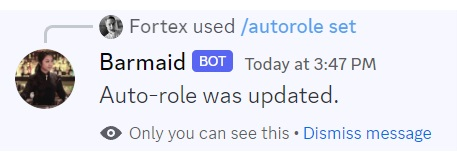
\includegraphics[scale=0.99]{autorole_set}
  \caption{\label{autorole_set}Ukázka nastavení automatické role}
\end{figure}

\begin{figure}[h!]
  \centering 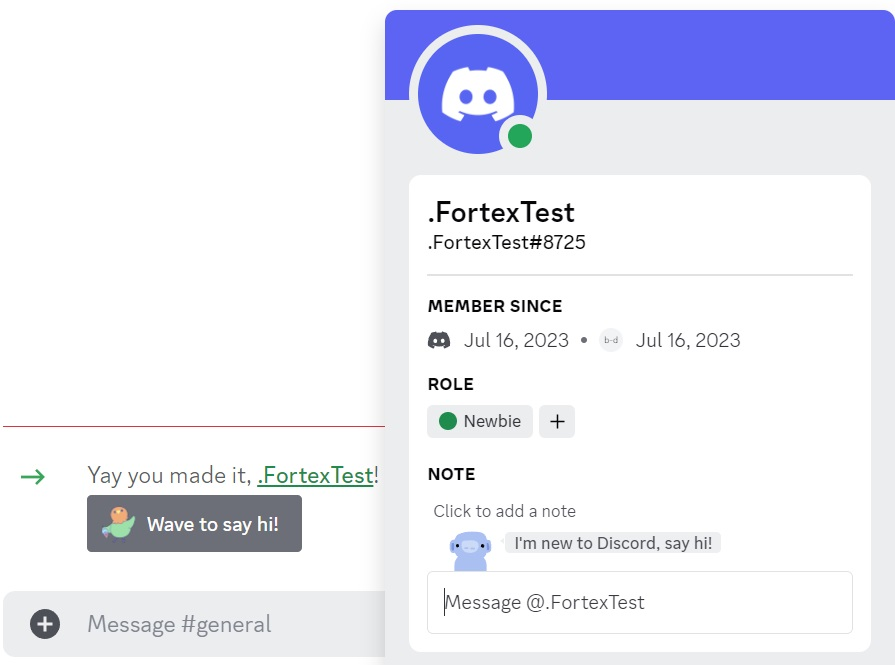
\includegraphics[scale=0.7]{autorole_given}
  \caption{\label{autorole_given}Ukázka automatického přidělení role}
\end{figure}

\newpage
\subsection{Události a jejich spravování}
Naplánování události je zajištěno pomocí příkazu {\it events echat}, zkratkou za \uv{events external chat}, 
tento příkaz vytvoří událost s definovaným jménem, popiskem, místem a datem konání a možnostmi uvádět celá jména
uživatelů při jejich evidenci nebo limit počtu uživatelů, kteří se mohou přihlásit. 
Zároveň s tím, pokud je definované
datum ve správném formátu, je automaticky vytvořeno oznámení 15 minut před počátkem události. Nerozpoznání datumu a času 
dává autorovi možnost mít zde libovolný text bez funkcionality oznámení předem. Příkaz je definovaný v modulu {\it event.py} ve složce {\it events}, která
zároveň definuje pohled {\it EventView}, kterým lze přidat tlačítka s určitou logikou ke zprávě a zaslat je společně.

\begin{figure}[h!]
  \centering 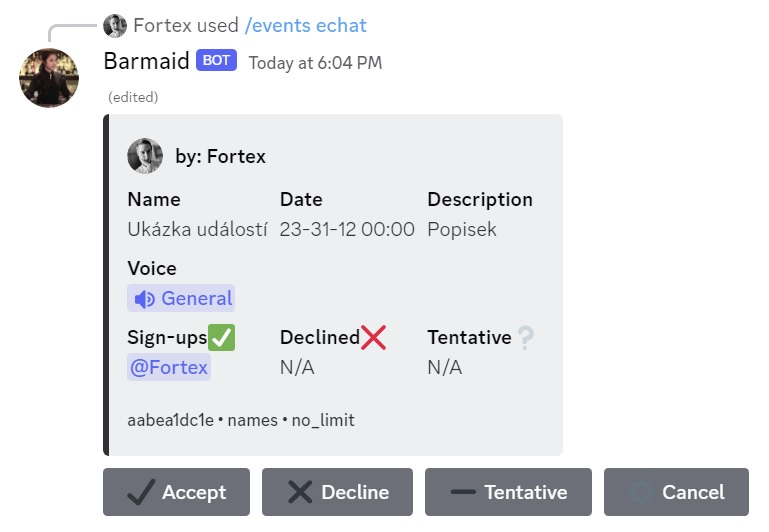
\includegraphics[scale=0.99]{eventukazka}
  \caption{\label{eventukazka}Ukázka vytvořené události příkazem {\it events echat}}
\end{figure}

Vytvořenou událost lze vidět na obr. \ref{eventukazka}, která je jako zapouzdřená zpráva
formátovaná do sloupců a řádků pro přehlednost. Pod samotnou zprávou jsou také tlačítka, které
k ní přísluší a intereagují. Tato tlačítka doplňují uživatele, který jej zmáčkl do příslušného
seznamu v události, tlačítko \uv{Cancel} slouží ke zrušení události a může ji využít pouze autor.
\newpage

Na zdrojovém kódu \ref{echat} je vidět mezi řádky č. 11 až 17, které definují
zapouzdřenou zprávu a formátují její položky (datum, místo, název apod.) do sloupců a řádků,
řádek č. 19 se stará o uložení do databáze. Nejpodstatnější je řádek č. 21, který odesílá
formátovou událost zapouzdřenou ve zprávě jako objekt třídy {\it discord.Embed} a
vlastními definovanými tlačítky třídou {\it EventView}. Na řádku č. 23 je
obsloužení a nastavení oznámení o události, je-li příkaz vhodně spuštěn s argumentem {\it start\_time}, který
respektuje určitý formát data a času.

\newpage
Funkce {\it setup\_notification} ze zdrojového kódu \ref{notification} je rozdělena do dvou částí,
první část se pokusí rozpoznat uživatelem stanovený čas, pokud se jedná o validní formát
a aktuální čas je déle než 15 minut před zahájením události, pozastaví se vykonávání této 
funkce o příslušný čas. Po jejím opětovném probuzení si zkontroluje obsah zprávy bota obsahující
událost, pokud existuje a nebyla zrušena, informuje do příslušného textového kanálu o tom, že se
událost blíží, rovněž vezme všechny uživatele jenž se mezitím na událost přihlásili a upozorní je
v soukromém chatu.

\begin{kicode}{python}{echat}{Část funkce pro vytvoření události}[h!]
  @events.command()
  async def echat(ctx:commands.Context, include_names:bool, 
                  title:str, description:str,
                  start_time:str, voice:VoiceChannel,
                  limit:int=0):
      # ... head of the function here

      # create buttons to message
      buttons = EventView()

      # embedded message for the event
      emb = Embed(color=int("0x2f3136", 0))
      emb.set_author(name=f"by: {ctx.author.display_name}", icon_url=ctx.author.avatar.url)
      emb.add_field(name="Name", value=title, inline=True)
      emb.add_field(name="Date", value=orignal_time, inline=True)
      emb.add_field(name="Description", value=description, inline=True)
      # ... rest of defition of all fields
      
      # ... saves the event into database

      event_message = await ctx.send(embed=emb, view=buttons)
      try:
          await setup_notification(ctx, emb, event_message.id, start_time)
      except ValueError:
          # ... error message about incorrect datetime for optional notifications
          await ctx.send(content=error_message,
                   delete_after=S.DELETE_COMMAND_ERROR, ephemeral=True)
\end{kicode}

\begin{kicode}{python}{notification}{Část funkce o oznámení události}[h!]
async def setup_notification(ctx:Context, emb:Embed, message_id:int, time:str):
    # ... try parse time into format, subtract 15 minutes
    # that time will be used to sleep the function
    
    # wait the desired time
    await asyncio.sleep(to_wait.seconds)
    
    # only notify if the event wasnt cancelled
    new_updated_message = await ctx.fetch_message(message_id)
    new_updated_embed = new_updated_message.embeds[0]
    event_name = new_updated_embed.fields[0]
    if not "Cancelled: " in event_name.value:
        # Notify in the channel
        await ctx.send(f"@here Event `{event_name.value}` starting soon!",
                    delete_after=S.DELETE_COMMAND_INVOKE)
        
        # Notify the signed up members
        # ... get the signed users
        for u in user_mentions:
            await u.send(f"Event `{event_name.value}` on `{ctx.guild.name}` is starting soon!")
\end{kicode}

\newpage
\subsection{Přehrávač}
O přehrávání audio stop se stará modul {\it music.py}, který zajišťuje kontrolu nad audiem a
samotné příkazy týkající se přehrávání audia. Modul obsahuje příkazy {\it stop}, {\it pause},
{\it resume} pro zastavení audia a odpojení bota z hlasového kanálu, pozastavení přehrávané skladby a 
opětovném pokračování v přehrávání. Příkazy {\it next}, {\it volume}, {\it queue}, {\it shazam}
slouží k přeskočení hudby, nastavení hlasitosti bota, zobrazení fronty audio obsahu v pořadí a zjištění
názvu audia. Pro zpracování playlistu slouží funkce {\it play\_playlist}, která dá do fronty
každý přístupný obsah z playlistu. Příkaz {\it play} přidá pouze jedno audio. Pokud se stane, že 
je některé audio právě přehráváné, tak bude zařazeno do stejné fronty jako používá příkaz {\it play\_playlist}.

\begin{figure}[h!]
  \centering 
\includegraphics[scale=0.99]{jukebox_play}
  \caption{\label{jukebox_play}Ukázka zaregistrování audia}
\end{figure}

\begin{figure}[h!]
  \centering 
\includegraphics[scale=1.2]{audio_playing}
  \caption{\label{audio_playing}Ukázka přehrávání audia botem}
\end{figure}

\newpage
Zdrojový kód \ref{play} ukazuje na řádcích č. 4-6 připojení bota do kanálu, kde se nachází autor příkazu,
řádek č. 8 obsluhu přehrávací fronty, na řádku č. 10 dochází k získání informací o audiu potřebné
například pro seznam fronty, řádky č. 13-19 sa postarají o spuštění audia pomocí funkce {\it play\_next}.

\begin{kicode}{python}{play}{Přehrání audia příkazem {\it play}}[h!]
  @commands.hybrid_command(with_app_command=True)
  @commands.guild_only()
  async def play(ctx:commands.Context, url:str):
      # ... get already connected client
      voice_client = await ctx.author.voice.channel
                      .connect(timeout=30, reconnect=True)
  
      # ... gets queue and puts the url into it
      
      # ... extracts the info about audio and processes it
  
      # start playing the next song if not already playing
      if not voice_client.is_playing():
          await play_next(ctx)
          await ctx.send("Jukebox started!",
                      delete_after=S.DELETE_EPHEMERAL)
          return
      await ctx.send("Added to queue!", 
                     delete_after=S.DELETE_EPHEMERAL)  
\end{kicode}

\newpage
Funkce ze zdrojového kódu \ref{playnext} zprostředkovává informace o aktuálně přehráváné hudbě
na řádku č. 2, na řádku č. 3 dochází k ukončení přehrávání je-li fronta vyčerpána, jinak
se z fronty získává odkaz audia (z platformy YouTube), který je následně zpracován na řádcích 5-9. 
Před odesláním k přehrání se provádí transformace audia do příslušné hlasitosti a formátu na řádku č. 10.
O samotné přehrání audia se poté starají řádky č. 12-14, které audio spustí v příslušném kanále komunitního serveru
a nastaví se po jeho ukončení opět na zavolání této funkce, kde právě přehrané audio už bylo odstraněno z fronty.


\begin{kicode}{python}{playnext}{Zprocesování a přehrání audia}[h!]
  async def play_next(ctx:commands.Context):
    # ... gets the url from queue
    # or stops playing when queue is empty
    
    loop = asyncio.get_event_loop()
    data = await loop.run_in_executor(None, lambda: _ytdl.extract_info(url, download=False))
    music = data["url"]
    
    player = discord.FFmpegPCMAudio(music, **_ffmpeg_options)
    # ... transforms the audio
        
    # ... gets the voice client
    voice_client.play(player, after=lambda e:
        asyncio.run_coroutine_threadsafe(play_next(ctx), loop=loop))
    # ... adds additional information to voice client
    # for example currently playing audio
\end{kicode}

\subsection{Hosting aplikace bota}
Pro nasazení aplikace je zvolena hostingová služba nazývající se Amazon Cloud Web Services \cite{aws} se
zvoleným hardwarem pronajatého stroje s jedním virtuálním procesorem a 1GB operační paměti běžící na operačním systému
Ubuntu 22.04 LTS, architektura 64-bit (x86). Tento způsob je zvolen na základě dostačujícího výkonu pro aplikaci bota
a použitím bezplatného účtu pro takto výpočetně nenáročný stroj. Se vzdáleným přístupem k tomuto stroji došlo k přesunutí
celé aplikace bota na tento stroj, kde jsou doinstalovány všechny potřebné prerekvizity podle přiloženého souboru {\it readme.txt}
u této aplikace, následně aplikace byla spuštěna.

% \subsection{Základní otestování funkcionalit}

% \subsubsection{Pravidla, pravomoce a kontrola členů}
% \subsubsection{Události}
% \subsubsection{Zvuk}

%%%  Po přeložení programem CSLaTeX (třikrát) je potřeba použít
%%%  program DVIPS a takto získaný PostScriptový soubor vytisknout
%%%  na PostScriptové tiskárně nebo pomocí programu GhostScript.
%%%
%%%  Rovněž je možné použít program DVIPDFM a vytvořit z dokumentu
%%%  soubor ve formátu PDF včetně hypertextových odkazů.


%%  'encoding=kódování' pro kódování tohoto a vložených zdrojových
%%  textů v kódování jiném než výchozím utf8

%%% Nepovinné argumenty `tables' a `figures' použijte pouze v případě,
%%% že váš dokument obsahuje tabulky a obrázky a chcete vytvořit
%%% jejich seznamy za obsahem.
%%%
%%% Argument `joinlists' způsobí zřetězení obsahu a seznamů tabulek a obrázků.
%%% Není-li použít, všechny seznamy jsou uvedeny na samostatných stránkách.


%% v případě tvorby rejstříku přeložit vygenerovaný soubor .idx
%% programem Makeindex a v případě tvorby seznamu zkratek spustit
%% program Makeglossaries s parametrem jméno souboru zdrojového textu
%% bez přípony a následně opět (dvakrát) přeložit zdrojový text
%% programem pdfLaTeX.


%% Závěry práce. V jazyce práce a anglicky. Text pro jiný než
%% nastavený jazyk práce (nepovinným parametrem language makra
%% \documentclass, výchozí český) se zadává použitím makra s uvedením
%% jazyka jako nepovinného parametru.
\begin{kiconclusions}
% tady budu muset napsat něco o tom že integrovaný discord eventy ještě nebyly
% když jsem měl téma bakalářky, ale během vývoje to tam přidali neboť je to
% fast growing app af

% že se povedlo napojit na YouTube API a používat ho, dalo by se napojit i na
% Spotify ale je otázkou ToS sdílením placené hudby (bot by měl premium spotify acc)

% a nakonec jako rozšíření by bylo supr zakomponovat do toho voice recognition
% když jsou uživatelé ve voice channels aby příkazy šli vyvolávat i hlasem a nejen
% přes psaný příkazy

% ne vše je v discord api a museli jsme sáhnout do rest api sami a to pro integrované discord
% eventy které v discord.py ve verzi 2.0.0 ještě nejsou přidané, to byl problém avšak se
% to povedlo

Cílem práce bylo vytvořit aplikaci bota pro platformu Discord, která umožní zlepšení
uživatelské zkušenosti na platformě správou komunity, správou uživatelů, plánováním událostí a zprostředkováním audio přehráváče.

Teoretická část práce obsahuje seznámení čtenáře s platformou Discord a její funkcionalitou. Popisuje 
technologie jenž platforma nabízí, jak fungují a jak se s nimi zachází. Popisuje také technologie, se kterými
aplikace bota pracuje navíc od samotných technologií platformy.

V praktické části je popsán návrh aplikace bota, který by měl umět ke splnit zadané požadavky a detailněji
popisuje jejich vlastnosti. Poté popisuje způsoby jakými byl návrh implementován a použit.

Výstupem práce je bot, který umožňuje moderátorům komunity na platformě Discord spravovat jejich komunitu způsoby
jako je přiřazení pravomocí pomocí vlastní definované role, kontrolou nově připojených uživatelů a jejich záznamů trestů, které má bot dostupné a sám
si je vytvořil. Umožňuje také stanovit pravidla platná pro komunitu a tyto pravidla automaticky zaslat nově příchozímu uživateli.
Bot umožňuje uskutečnit události, které jsou naplánovány pomocí příkazu a jsou zobrazeny a evidovány přímo v chatu. Uživatelé 
se na tuto událost mohou přihlásit a budou moci být upozorněni před počátkem konání. Aplikace umožňuje 
také zlepšení uživatelské zkušenosti audio-přehrávačem ve hlasovém hovoru v kanálech komunity.
\end{kiconclusions}

\begin{kiconclusions}[english]
Goal of this thesis was to create an application for Discord platform, which allows its users to enhance their
experience on the platform with better management of the guild communities and its members, mediate an events organizator and
audio player.

Theoretical part of the thesis contains an introduction to the Discord platform and its functionality. Description of technologies
which the platform offers, how they work and how to use them. It also describes technologies which the application uses
in addition to the platform itself.

The practical part describes the design of the application, which should be able to meet the requirements and more
detailed description of its features, then there are described the ways in which the design was implemented.

The output of the thesis is a bot, which allows moderators of the communities on the Discord platform to manage their
community in ways such as assigning privilages using their own defined role. Checking newly connected users and their
punishments records, which the bot has available and created for himself before. Allowing to create own set of rules for the community and
automatically send them out to new users. The bot allows to create and hold for events, which are planned using a
command and are displayed directly in the chat, users can register for this event and
can be notified before the start of the event. The application also allows for an audio player in a voice channel in the
guild community to improve the user experience.
\end{kiconclusions}

%% Přílohy obsahu textu práce, za makrem \appendix.
\appendix

%% Obsah přiloženého datového média. Poslední příloha. Upravte podle vlastní
%% práce!
\section{Obsah přiloženého datového média} \label{sec:ObsahMedia}

\begin{description}

\item[\texttt{theses/}] \hfill \\
  Kompletní text této práce v PDF formátu.

\item[\texttt{src/}] \hfill \\
  Kompletní zdrojové soubory implementované aplikace, jejími konfiguračními soubory
  a souborem obsahující všechny knihovny třetích stran pro jejich instalaci
  skrze program {\ pip}, dostupný po nainstalování interpretu programovacího
  jazyka popsaném v souboru s instrukcemi readme.txt. 

\item[\texttt{readme.txt}] \hfill \\
  Instrukce pro instalaci a~spuštění programu {\it barmaid.py}, včetně
  všech požadavků pro jeho bezproblémový provoz. / Instrukce a~webová adresa, na
  které je aplikace nasazena pro účel testování při tvorbě posudků
  práce a~pro účel obhajoby práce.

\end{description}


%% -------------------------------------------------------------------

%% Sazba volitelného seznamu zkratek, za přílohami.
% \printglossary[type=\acronymtype]
\printglossary
% \printnoidxglossaries

%% Sazba povinné bibliografie, za přílohami (případně i za seznamem
%% zkratek). Při použití BibLaTeXu použijte makro
%% \printbibliography. jinak prostředí thebibliography. Ne obojí!

%% Sazba i v textu necitovaných zdrojů, při použití
%% BibLaTeXu. Volitelné.
\nocite{*}
%% Vlastní sazba bibliografie při použití BibLaTeXu.
% \printbibliography

% Bibliografie, včetně sazby, při nepoužití BibLaTeXu.
\begin{thebibliography}{99}
\bibitem{ffxiv} Wikipedia. {\it Final Fantasy XIV.} [online]. 2013. [cit. 2023-16-03]. Dostupné z: \url{https://en.wikipedia.org/wiki/Final_Fantasy_XIV}
\bibitem{dc} Wikipedia. {\it Discord.} [online]. 2014. [cit. 2023-16-03]. Dostupné z: \url{https://en.wikipedia.org/wiki/Discord}
\bibitem{porovnani} Chanty. {\it Slack vs Discord – Gaming, Working or Both?} [online]. 2022. [cit. 2023-16-03]. Dostupné z: \url{https://www.chanty.com/blog/discord-vs-slack/}
\bibitem{rate} Discord. {\it Rate Limits.} [online]. 2015. [cit. 2023-17-03]. Dostupné z: \url{https://discord.com/developers/docs/topics/rate-limits}
\bibitem{discordapi} Discord. {\it Discord API.} [online]. 2015. [cit. 2023-17-03]. Dostupné z: \url{https://discord.com/developers/docs/reference#api-reference}
\bibitem{webapi} Discord. {\it Gateway.} [online]. 2015. [cit. 2023-17-03]. Dostupné z: \url{https://discord.com/developers/docs/topics/gateway}
\bibitem{restapi} Toptal. {\it How to Make a Discord Bot: an Overview and Tutorial.} [online]. 2010-2023. [cit. 2023-17-03]. Dostupné z: \url{https://www.toptal.com/chatbot/how-to-make-a-discord-bot}
\bibitem{asyncio} Caleb Hattingh. {\it Using Asyncio in Python.} O'Reilly Media, Incorporated, 2020. ISBN 978-149-2075-332
\bibitem{discordpy} Github. {\it discord.py.} [online]. 2023. [cit. 2023-18-03]. Dostupné z: \url{https://github.com/Rapptz/discord.py}
\bibitem{rpi} Raspberry. {\it Computing for everybody.} [online]. 2012. [cit. 2023-18-03]. Dostupné z: \url{https://www.raspberrypi.com/}
\bibitem{aws} Amazon. {\it What is cloud computing?} [online]. 2006. [cit. 2023-18-03]. Dostupné z: \url{https://aws.amazon.com/what-is-cloud-computing/}
\bibitem{libs} Discord. {\it Community Resources.} [online]. 2015. [cit. 2023-18-03]. Dostupné z: \url{https://discord.com/developers/docs/topics/community-resources#libraries}
% \bibitem{asyncio} Python Tutorial. {\it Python Event Loop.} [online]. 2023. [cit. 2023-18-03]. Dostupné z: \url{https://www.pythontutorial.net/python-concurrency/python-event-loop/}
\bibitem{loop} Interactive Bees Blog. {\it Asyncio - vylepšené asynchronní paradigma.} [online]. 2022. [cit. 2023-18-03]. Dostupné z: \url{https://blog.neonkid.xyz/283}
\bibitem{ffmpeg} Wikipedia. {\it FFmpeg.} [online]. 2007. [cit. 2023-18-03]. Dostupné z: \url{https://cs.wikipedia.org/wiki/FFmpeg}
\bibitem{ffmpeg2} FFmpeg. {\it Ffmpeg.} [online]. 2023. [cit. 2023-18-03]. Dostupné z: \url{https://ffmpeg.org/}

\end{thebibliography}

%% Sazba volitelného rejstříku, za bibliografií.
\printindex

\end{document}

%%% Local Variables:
%%% mode: latex
%%% TeX-master: t
%%% End:
